\section{商业模式类型}
所关注的五种商业模式类型:
\begin{itemize}
    \item 分拆商业模式
    \item 长尾商业模式
    \item 多边平台商业模式
    \item 免费商业模式
    \item 开放式商业模式
\end{itemize}

\subsection{分拆商业模式}

企业内部存在三类规则:经济、竞争与文化规则
\begin{itemize}
    \item 由此可以区分三种活动:客户关系管理、新产品开发、基础设施管理
    \item 上述三种活动对应三种价值信条:亲近顾客、产品领先、运营卓越
    \item 但这三类活动驱动因素不同,彼此之间冲突,企业内部存在不必要的消长
    \begin{itemize}
        \item 解决办法:分拆,各自独立
    \end{itemize}
\end{itemize}

\begin{table}[H]
    \centering
    \resizebox{\textwidth}{!}{
    \begin{tabular}{|l|l|l|l|}
    \hline
         & \multicolumn{1}{c|}{新产品开发}                                          & \multicolumn{1}{c|}{客户关系管理}                                                   & \multicolumn{1}{c|}{基础设施管理}                                                  \\ \hline
    经济规则 & \begin{tabular}[c]{@{}l@{}}早期市场进入获得高溢价和\\ 大量市场份额:速度是关键\end{tabular} & \begin{tabular}[c]{@{}l@{}}高昂的客户开发成本要求从\\ 每个客户手中获取高份额:\\ 范围经济是关键\end{tabular} & \begin{tabular}[c]{@{}l@{}}高固定成本使得高产量成为获\\ 得低单位成本的关键:规模经\\ 济是关键\end{tabular} \\ \hline
    竞争规则 & \begin{tabular}[c]{@{}l@{}}能力之争,进入门槛低:大\\ 量小玩家争奇斗艳\end{tabular}     & \begin{tabular}[c]{@{}l@{}}范围之争:少量的大玩家主\\ 导市场\end{tabular}                    & \begin{tabular}[c]{@{}l@{}}规模之争:迅速固化的市场;\\ 少量大玩家主导市场\end{tabular}            \\ \hline
    文化规则 & \begin{tabular}[c]{@{}l@{}}以雇员为中心:呵护创意明\\ 星\end{tabular}            & \begin{tabular}[c]{@{}l@{}}高度服务导向:顾客第一心\\ 态\end{tabular}                      & \begin{tabular}[c]{@{}l@{}}聚焦成本:强调标准化、可预\\ 期性和生产效率\end{tabular}              \\ \hline
    \end{tabular}
    }
    \end{table}

    \subsubsection{传统私人银行商业模式及其中的消长}
    \begin{figure}[H]
		\centering
        \vspace{-0.5em}
		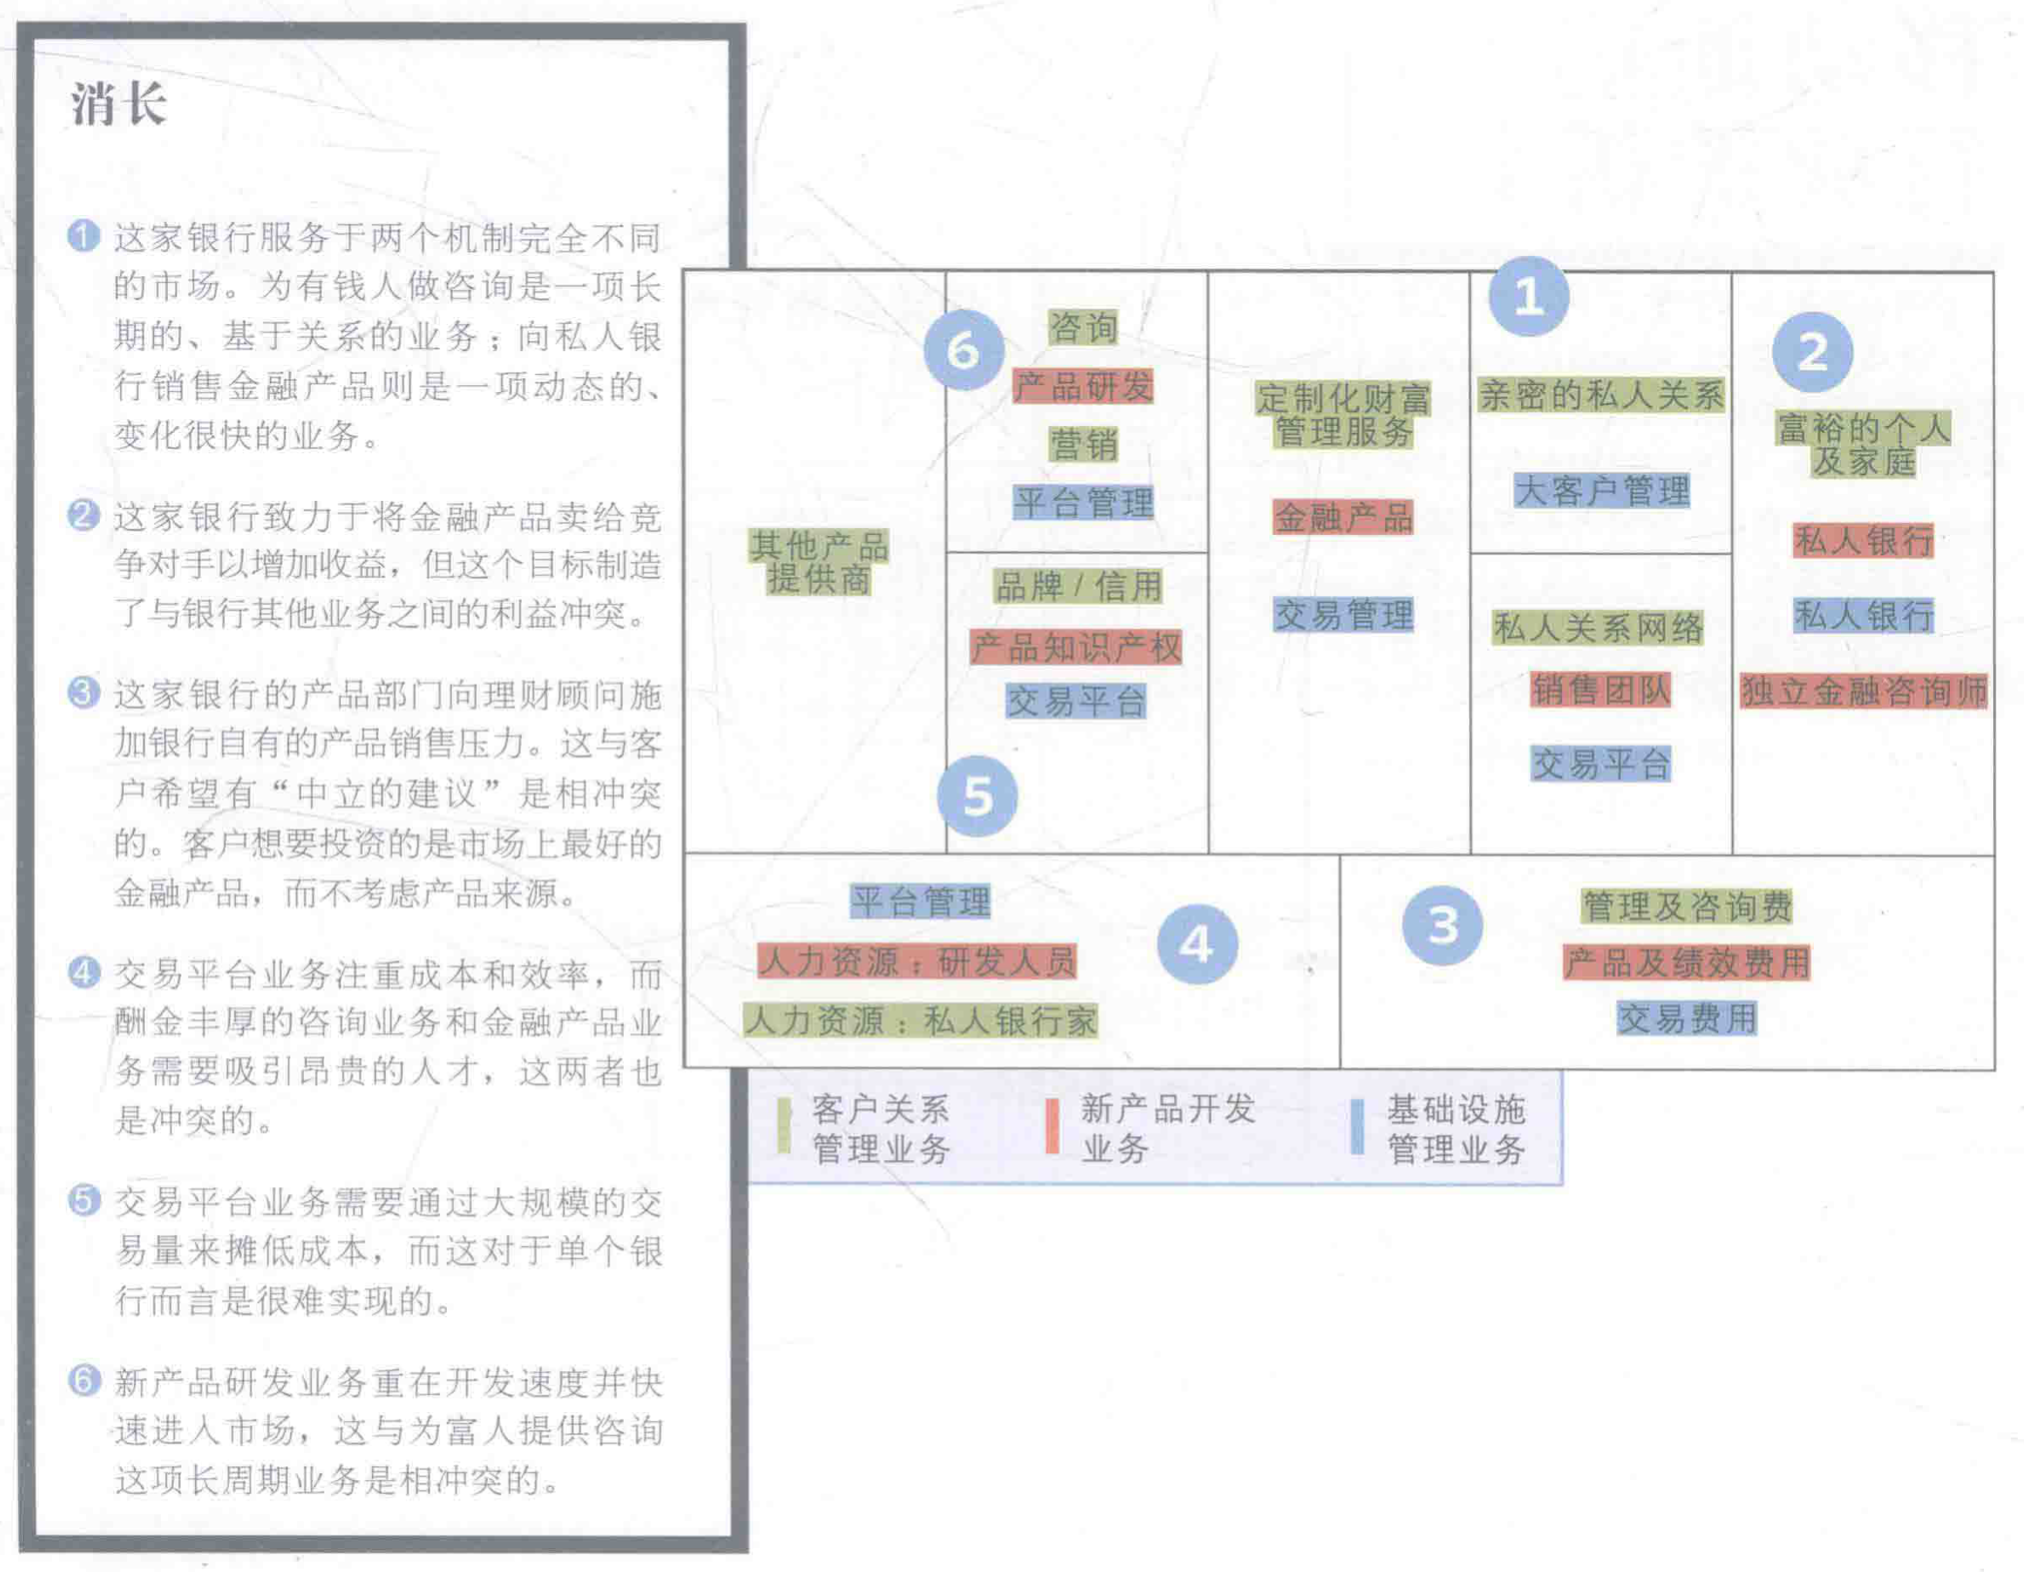
\includegraphics[width=0.95\textwidth]{img/传统私人银行商业模式及其中的消长.png}
        \vspace{-0.5em}
	\end{figure}


    \subsubsection{移动通信行业的拆分}
    移动通信企业已经为自己的商业模式松绑。传统的移动通信企业针对网络质量展开竟争,而现在它们却与竞争对手达成网络共享协议或者将网络运营业务外包给设备生产厂家。因为它们意识到它们的核心资产已经不再是网络本身,而是它们的品牌和客户关系。
    \begin{figure}[H]
		\centering
        \vspace{-0.5em}
		\includegraphics[width=\textwidth]{img/移动通信行业的拆分.png}
        \vspace{-0.5em}
	\end{figure}

    拆分后三个独立的商业模式
    \begin{figure}[H]
		\centering
        \vspace{-0.5em}
		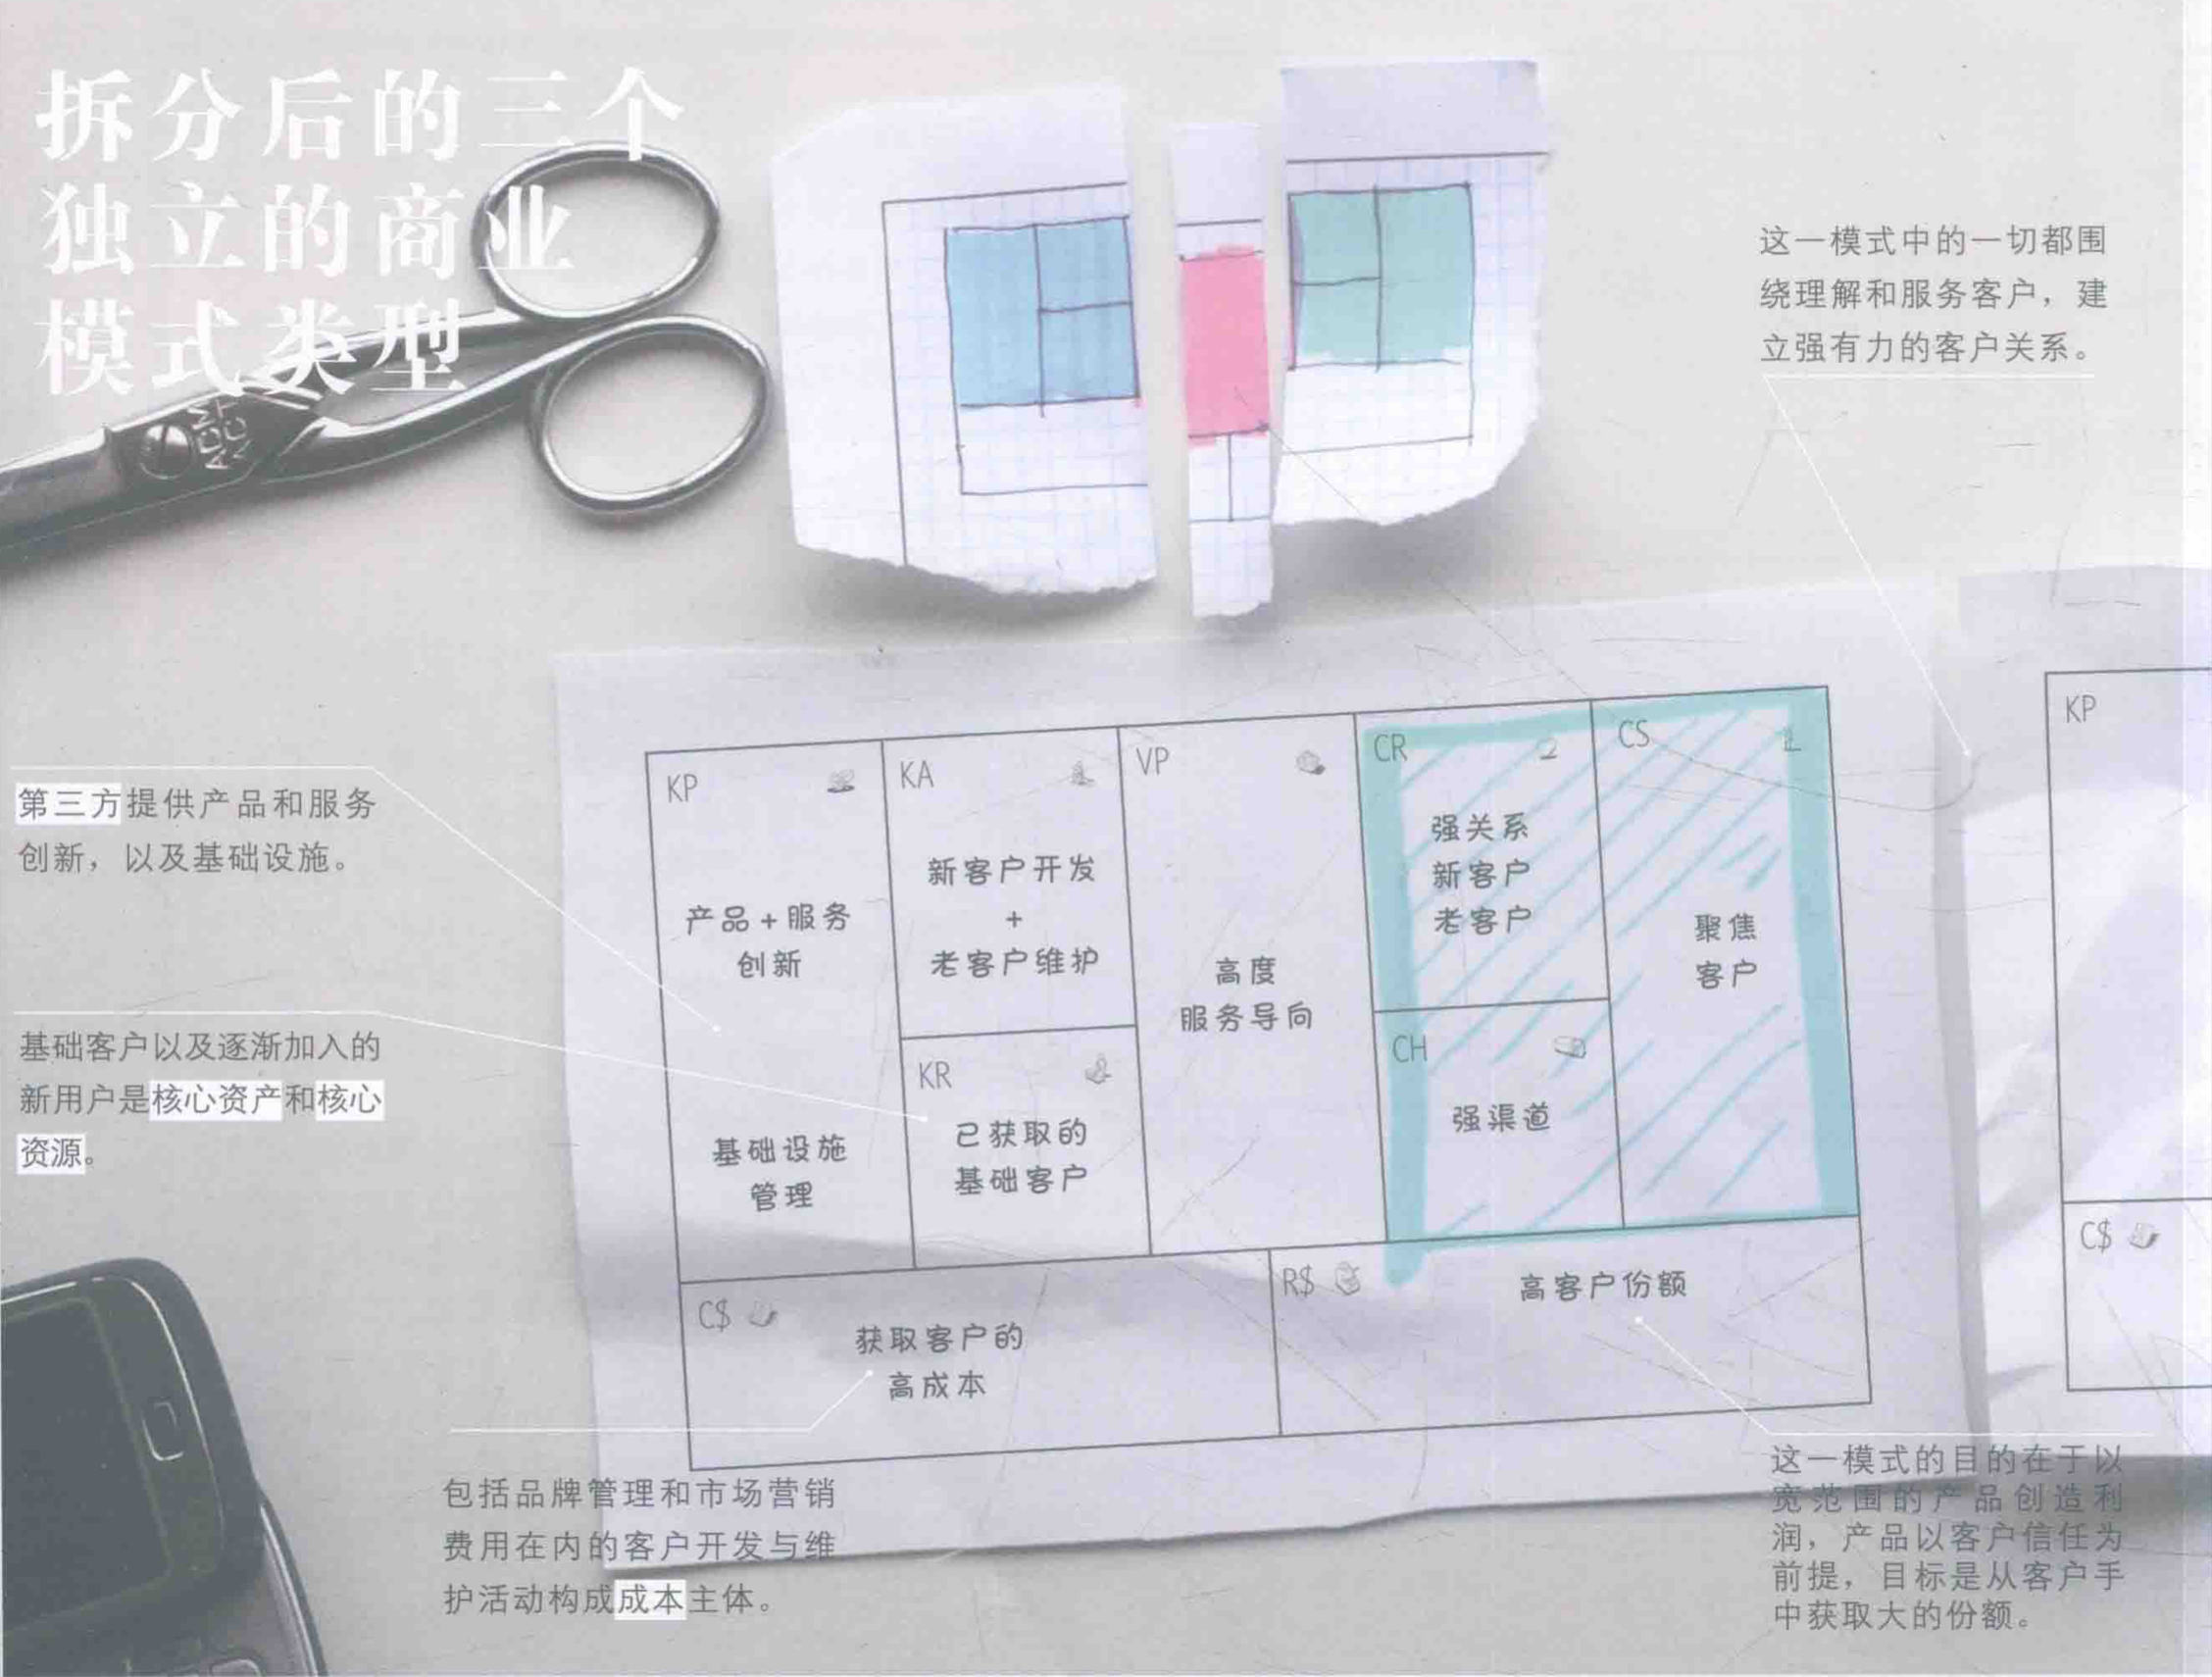
\includegraphics[width=\textwidth]{img/拆分后三个独立的商业模式1.png}
        \vspace{-0.5em}
	\end{figure}

    \begin{figure}[H]
		\centering
        \vspace{-0.5em}
		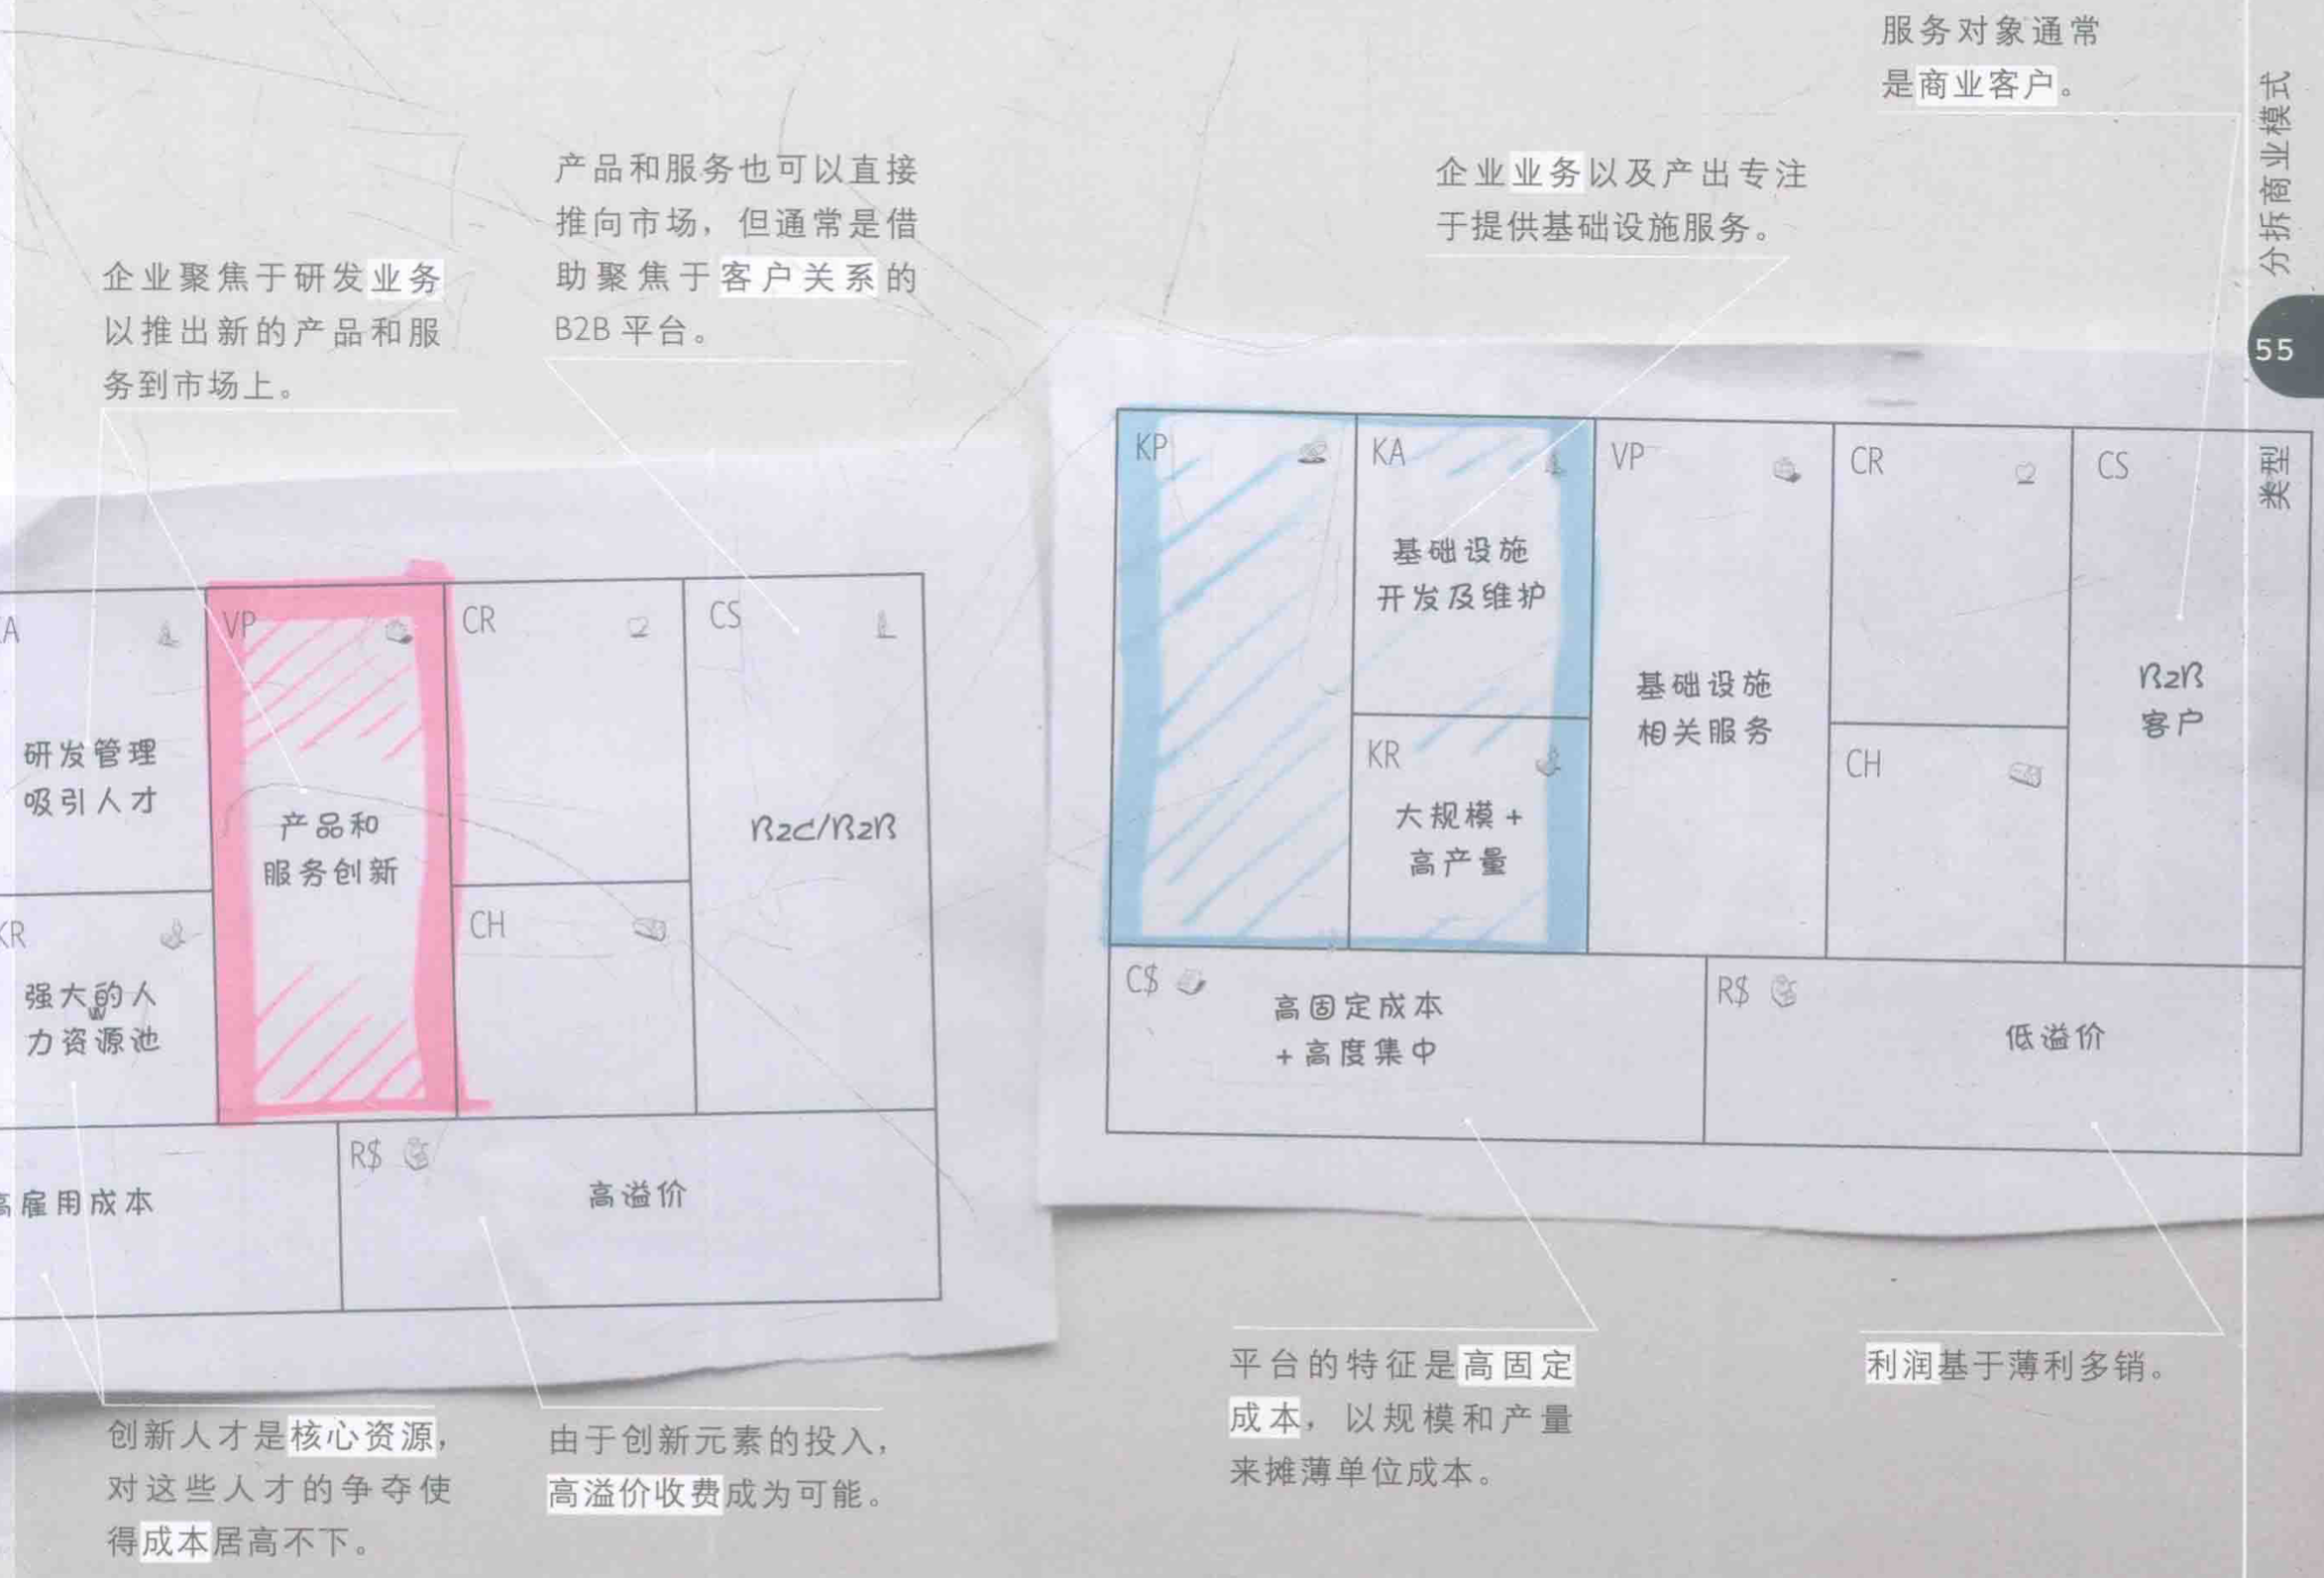
\includegraphics[width=\textwidth]{img/拆分后三个独立的商业模式2.png}
        \vspace{-0.5em}
	\end{figure}

    \subsection{长尾商业模式}
    长尾商业模式在于少量多种地销售自己的产品:它致力于提供相当多种类的小众产品,而其中的每一种卖出量相对很少。
    \begin{itemize}
        \item 将这些小众产品的销售汇总,所得收入可以像传统模式销售所得一样可观,它不同于传统模式,以销售少数的明星产品负担起绝大部分的收益。
        \item 长尾商业模式要求低库存成本以及强大的平台以保证小众商品能够及时被感兴趣的买家获得。
    \end{itemize}

    \begin{figure}[H]
		\centering
        \vspace{-0.5em}
		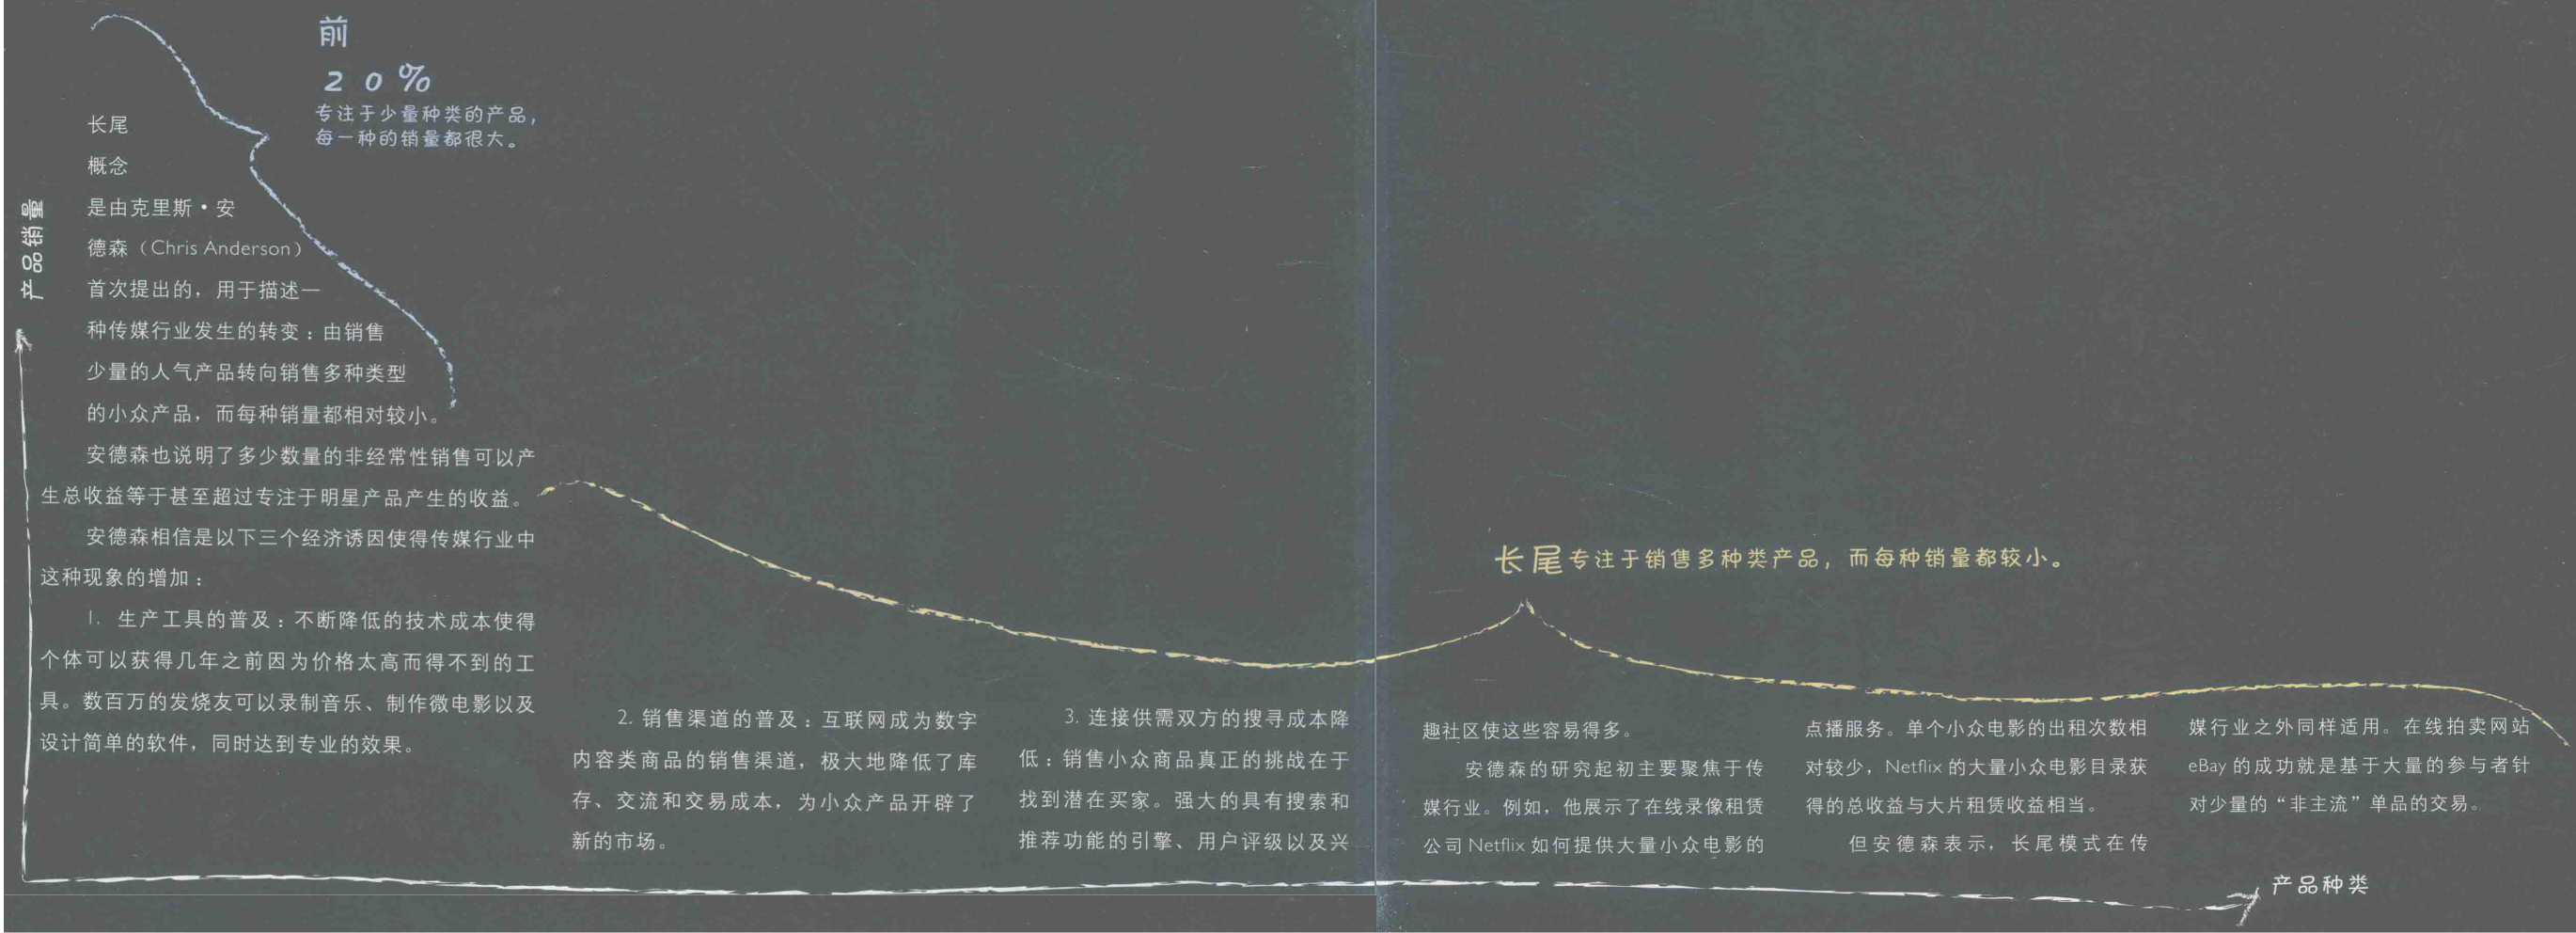
\includegraphics[width=\textwidth]{img/长尾概念的提出.png}
        \vspace{-0.5em}
	\end{figure}

    \subsubsection{图书出版行业的转型}
    \begin{figure}[H]
		\centering
        \vspace{-0.5em}
		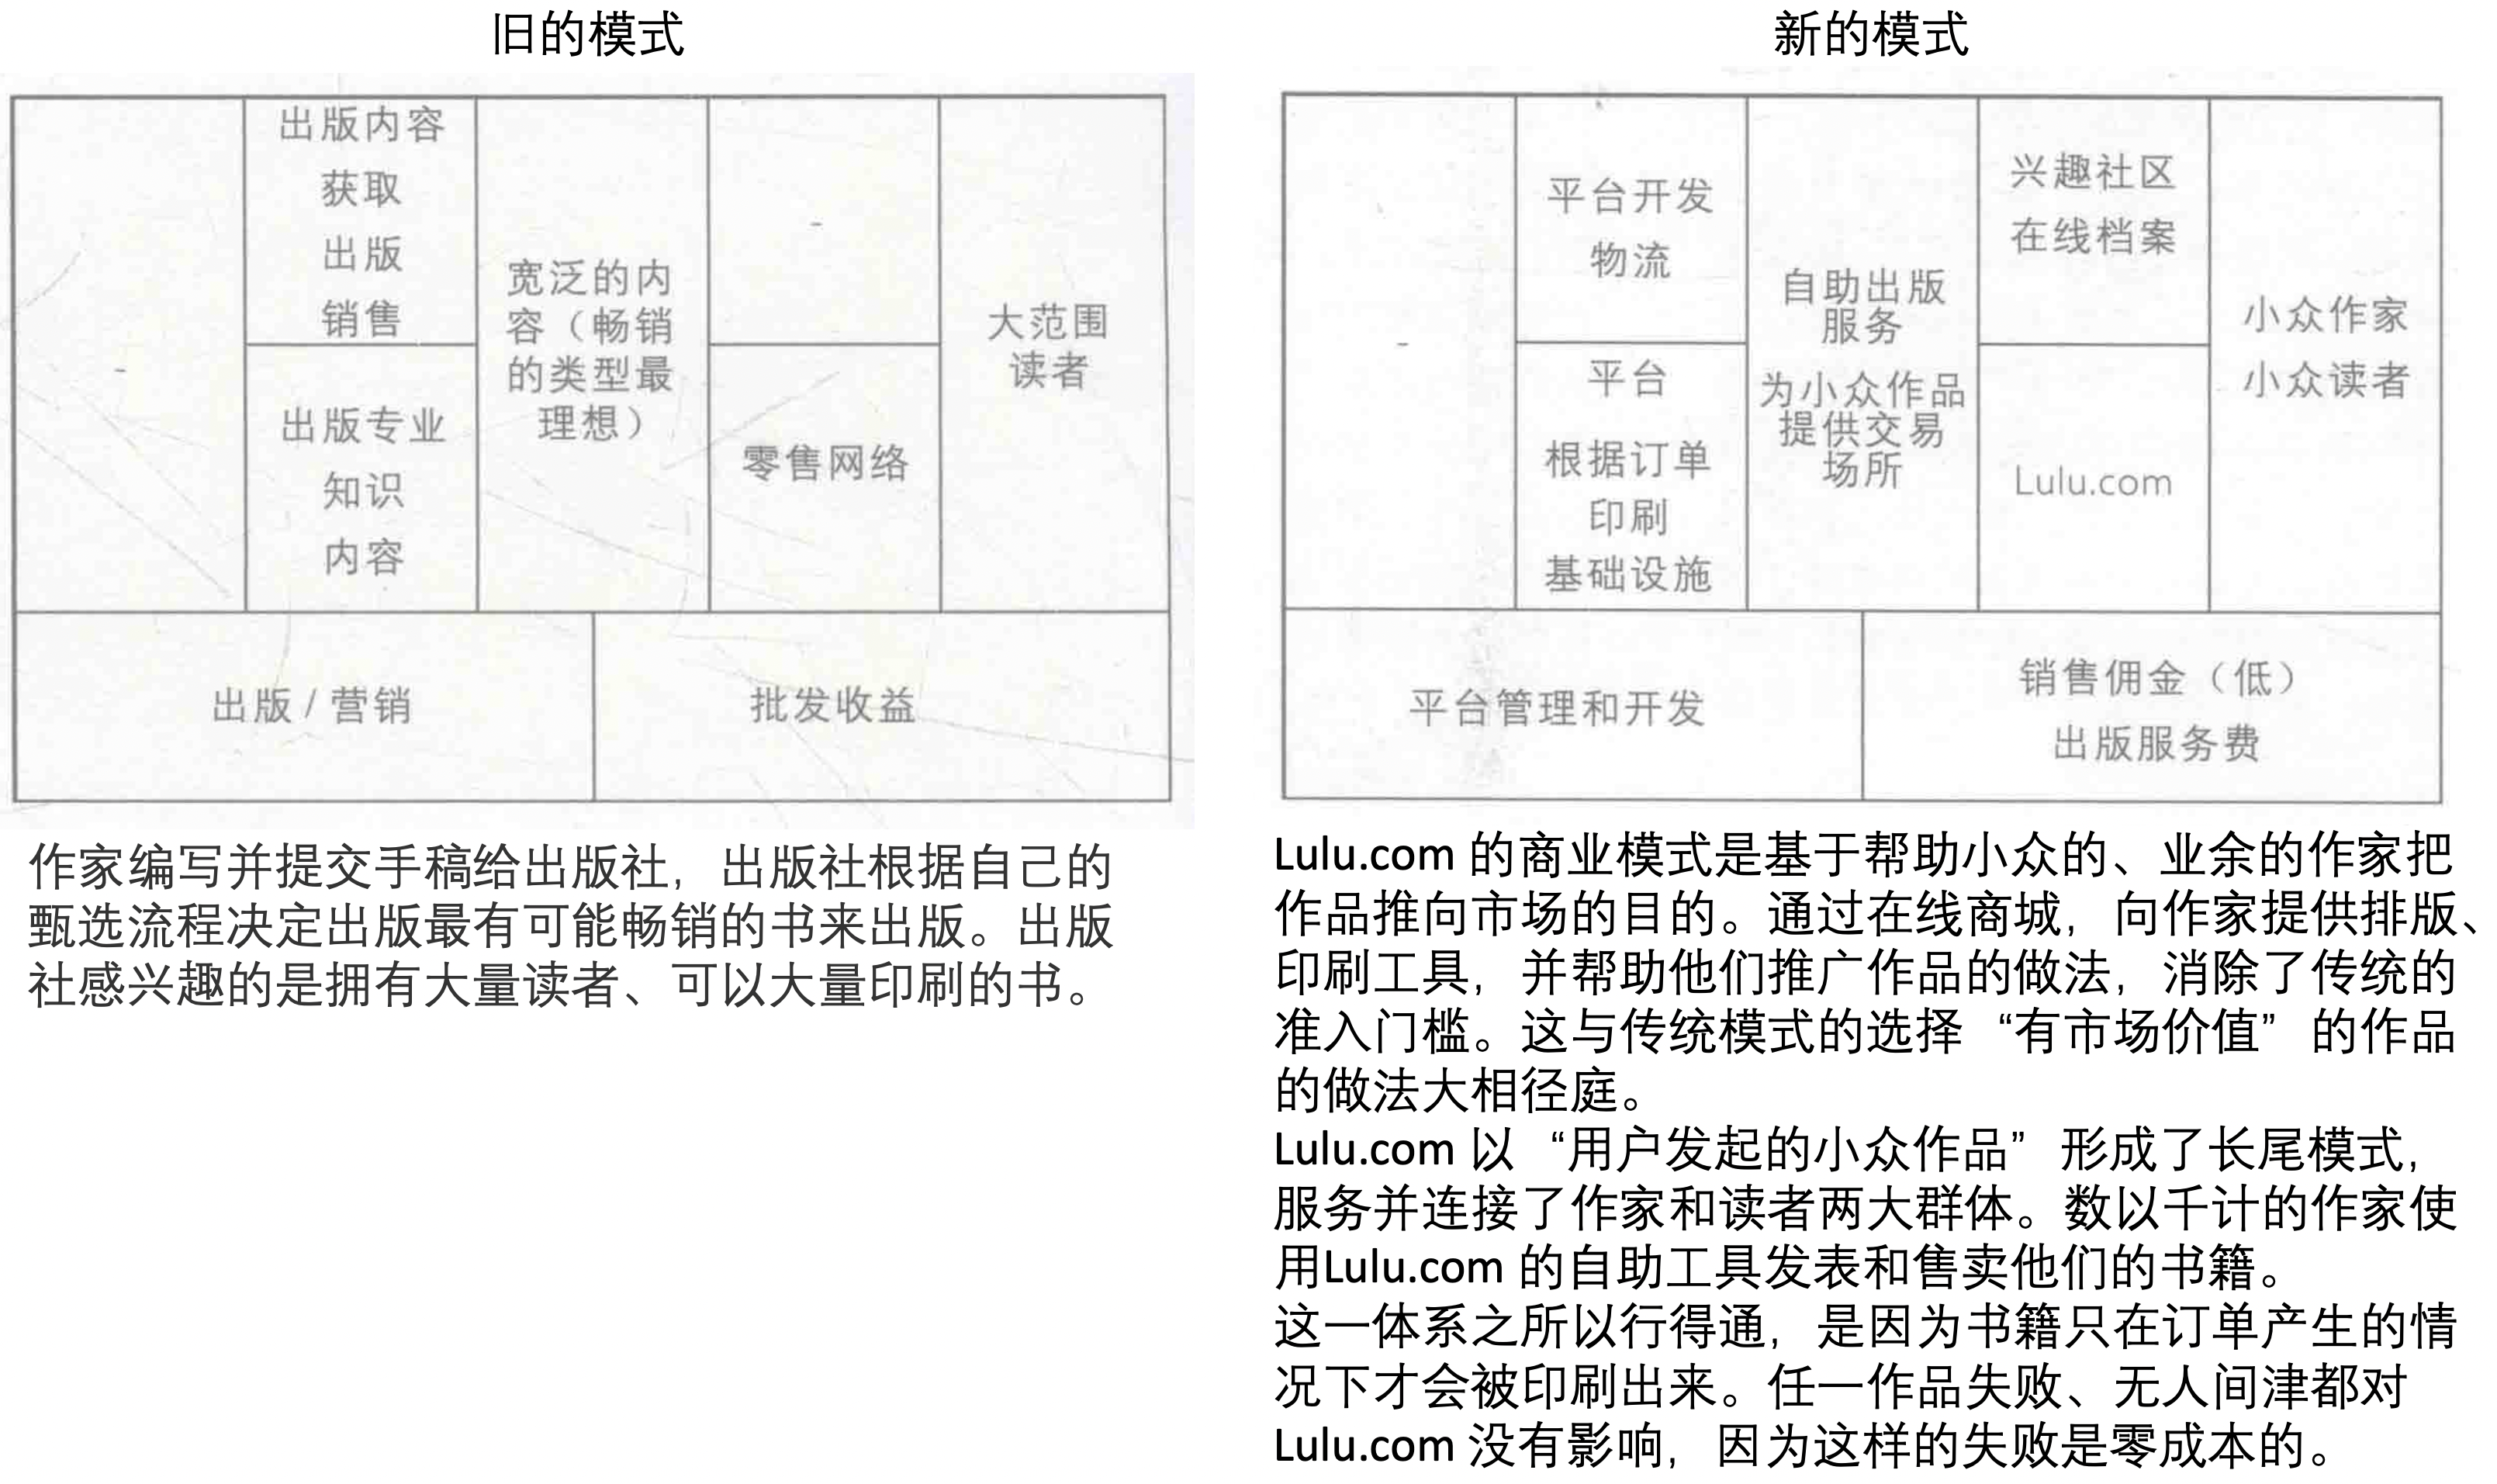
\includegraphics[width=\textwidth]{img/图书出版行业的转型.png}
        \vspace{-0.5em}
	\end{figure}

    \subsubsection{乐高的新长尾模式}
    2005年,乐高开始推出用户定制套餐——乐高工厂,允许客户使用在线设计软件,甚至允许用户选择包装盒子,让用户成为了乐高设计体验的主动参与者。
    \begin{figure}[H]
		\centering
        \vspace{-0.5em}
		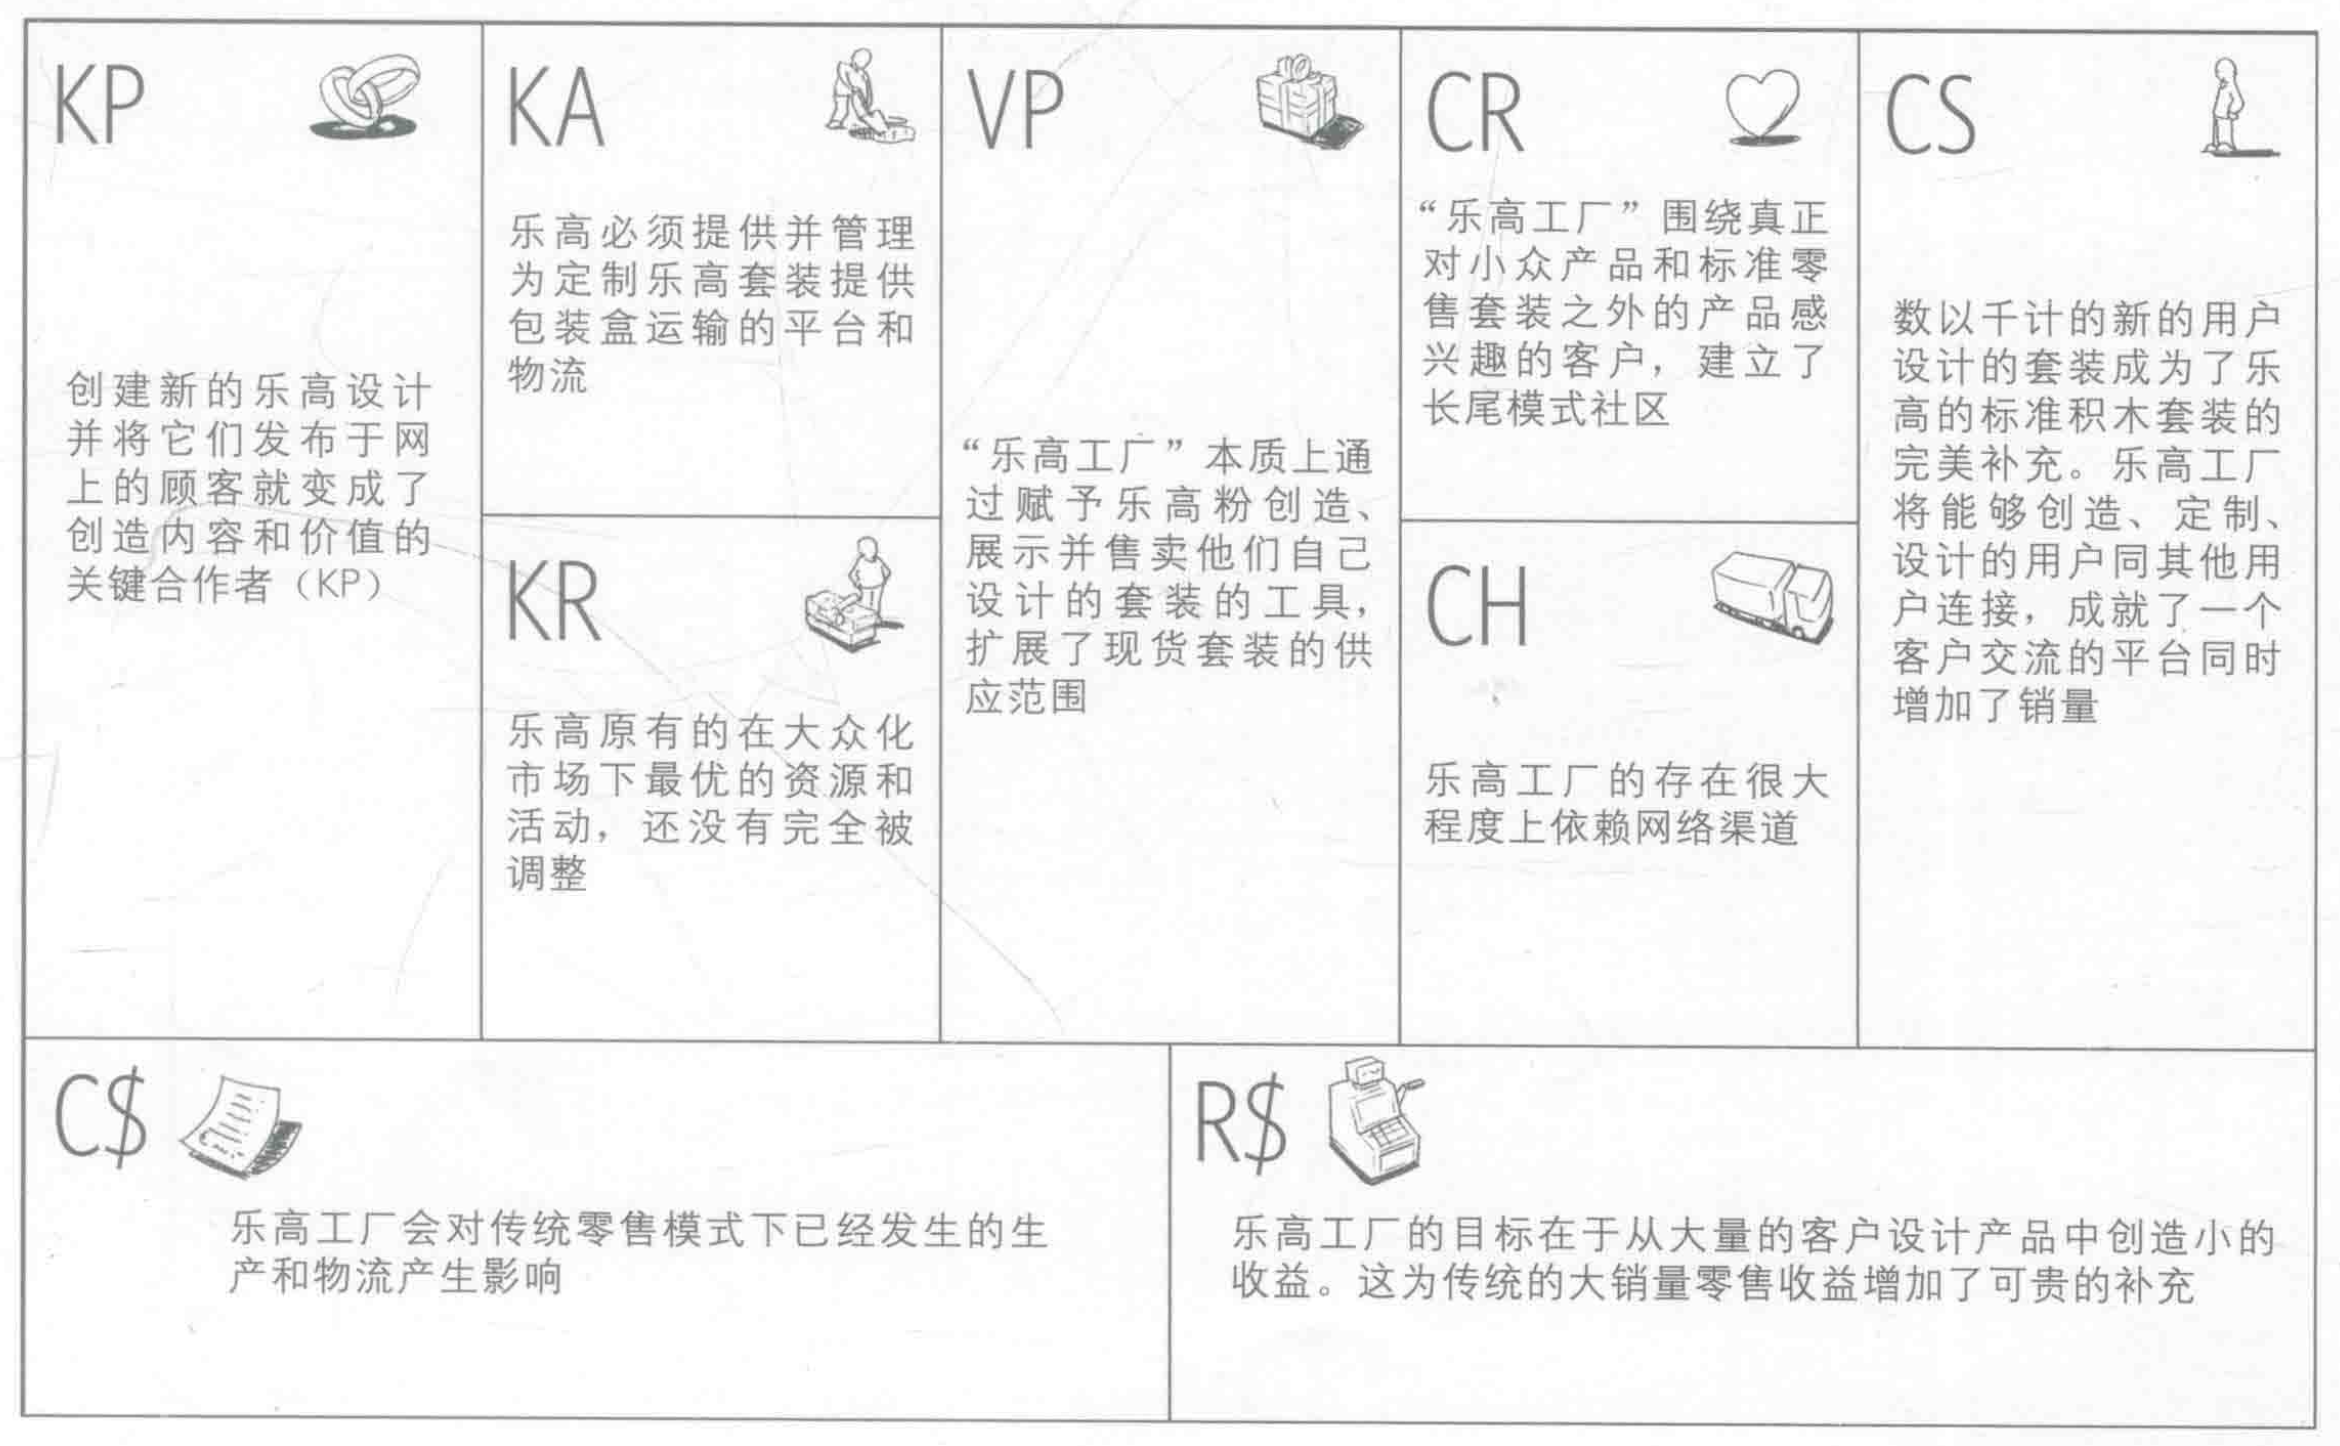
\includegraphics[width=\textwidth]{img/乐高的新长尾模式.png}
        \vspace{-0.5em}
	\end{figure}

    \subsubsection{长尾模式的流行原因与发展趋势}
    大量行业都有“长尾”的趋势
    \begin{itemize}
        \item 个人主义流行与社会物资丰富导致的需求释放
        \item 人类社会中的流行因素与趋势三年一小变、五年一大变
        \item 生产设计与渠道营销在效率上的不断提升带来的产销能力工具化、服务化
        \item 互联网技术不断发展导致的供需双方匹配更加便利
        \item 复用生产和渠道,可以和热销品并存(长尾模式背后往往有大公司的影子)
    \end{itemize}

    长尾模式的共性与发展趋势
    \begin{itemize}
        \item 对生产环节(含渠道)的标准化程度要求较高(媒体、影视、游戏、一般日用品)
        \item 生产设计环节一般仍依赖于大型厂家,渠道依赖互联网(社区也可能是创意、构思的来源)
        \item “长尾之后”:突破因传统生产、设计、营销导致的二八曲线,长尾部分扁平化;形成若干“小众中心”,并分别向“大众中心”转化
    \end{itemize}

    \begin{figure}[H]
		\centering
        \vspace{-0.5em}
		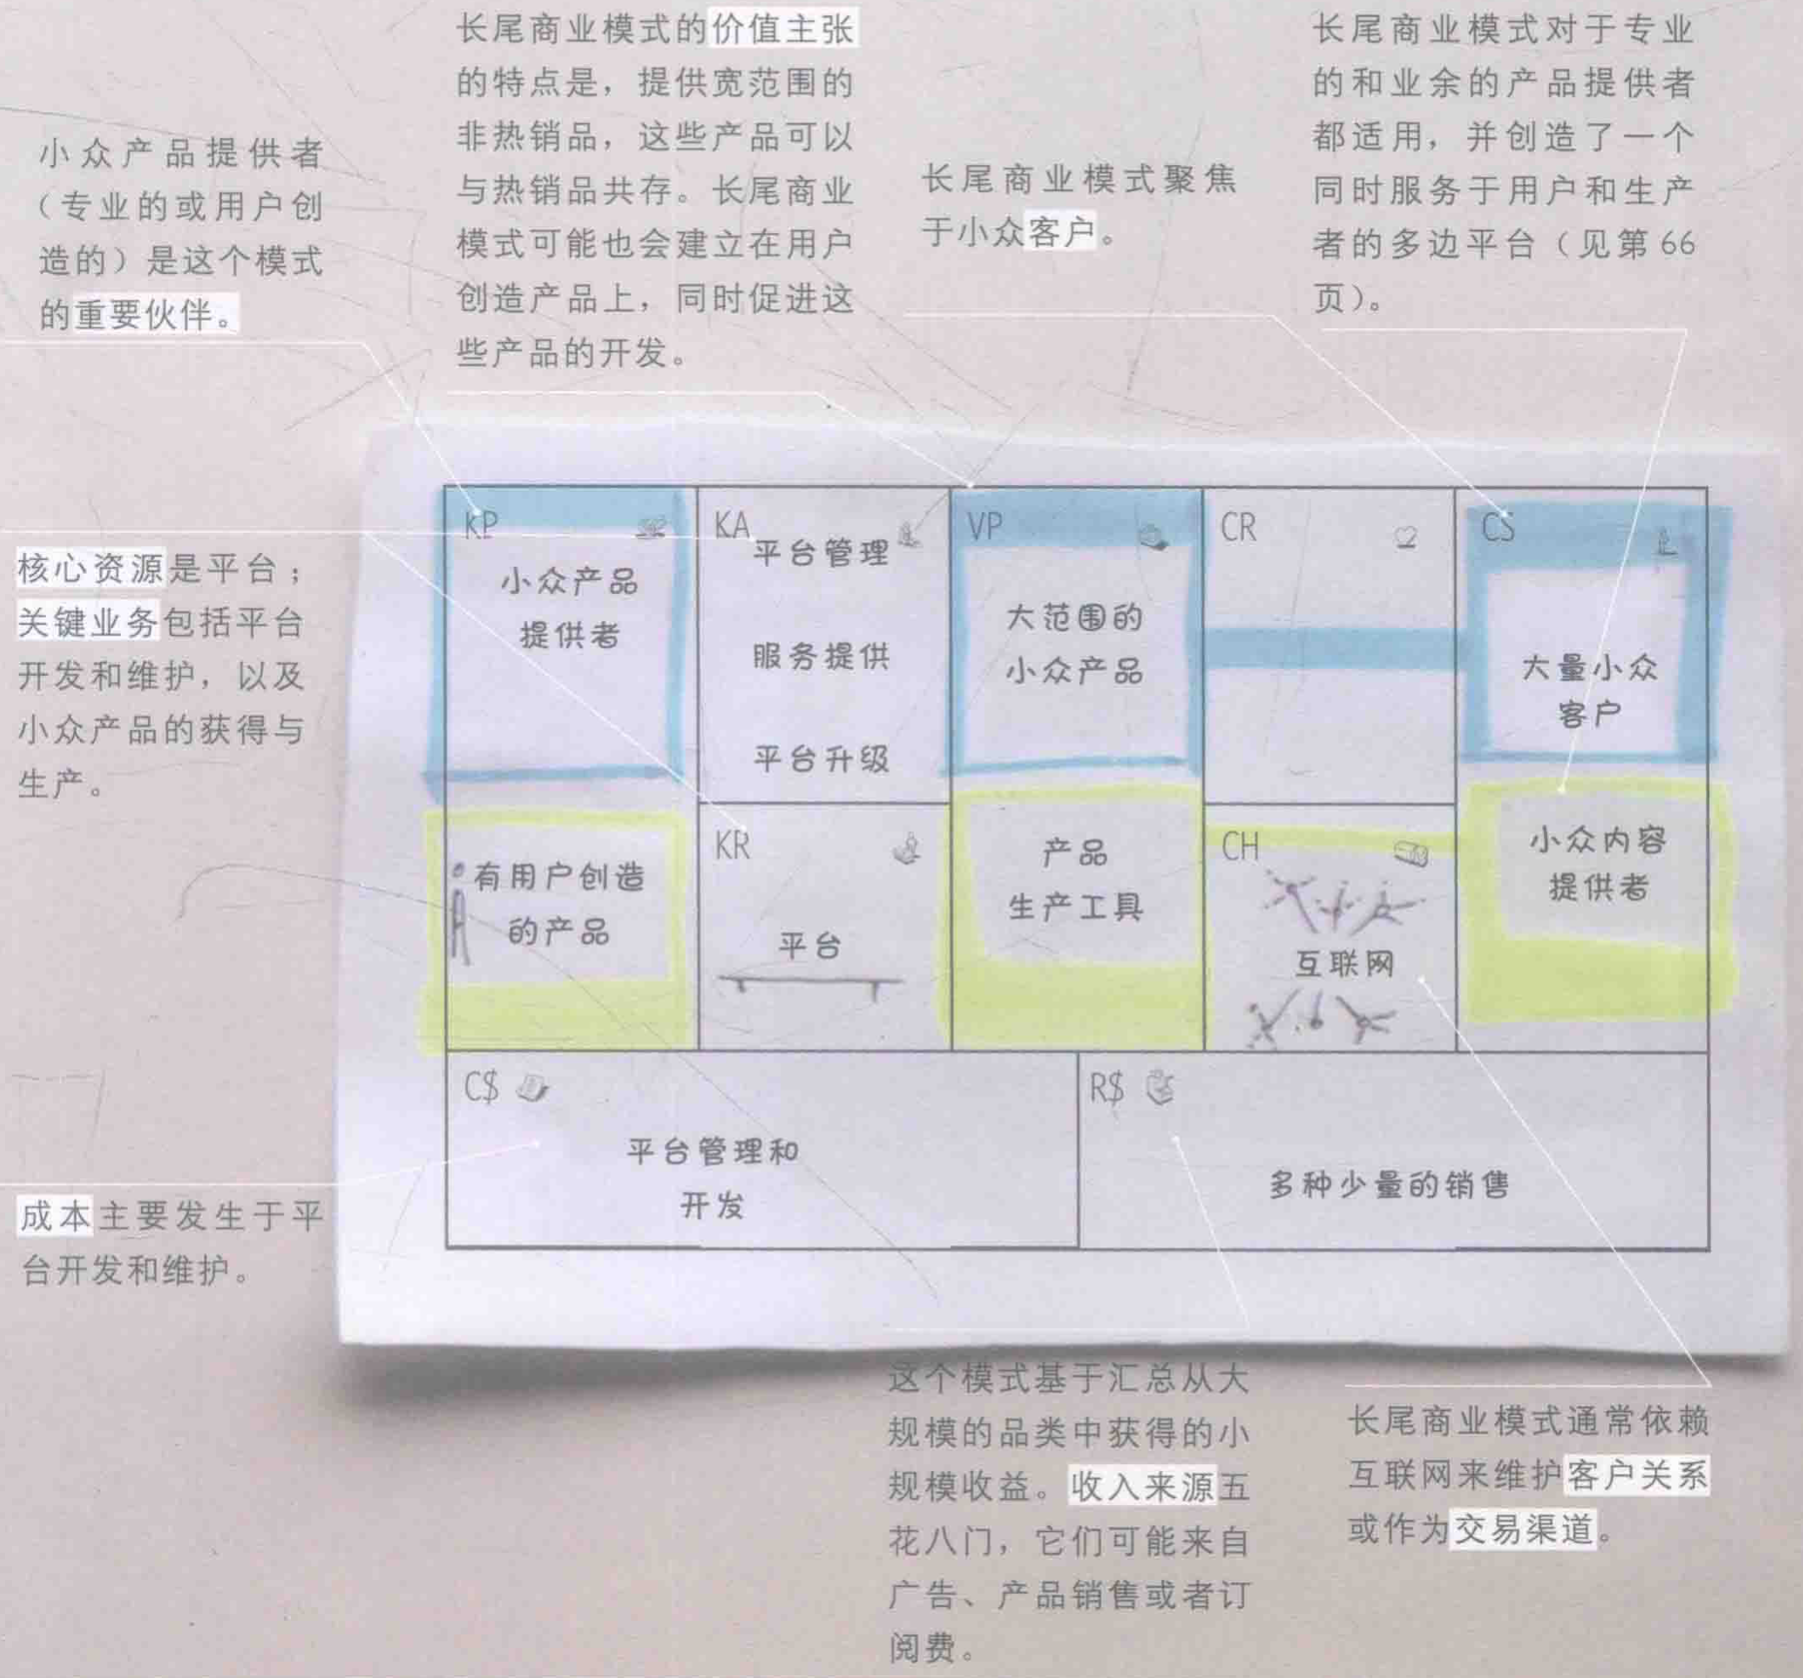
\includegraphics[width=0.85\textwidth]{img/长尾模式总结.png}
        \vspace{-0.5em}
	\end{figure}

    \subsection{多边平台商业模式}
    多边平台(多边市场)是将两个或更多独立但相互依存的客户群体连接在一起的平台。
    \begin{itemize}
        \item 这样的平台对于平台中某一群体的价值在于平台中其他客户群体的存在。平台通过促进不同群体间的互动而创造价值,例如信用卡将商家和持卡人连接。
        \item 多边平台的价值提升在于它所吸引的用户数量的增加,这种现象被称为网络效应。
        \item 平台对于单个用户群体的价值本质上取决于平台中“另一群体”的用户数量,例如游戏开发商之所以会为某一个电子游戏设备开发新游戏是因为已经有大量的玩家在使用它。
        \item 多边平台经常会面临一个“先有鸡还是先有蛋”的两难困境。
        \begin{itemize}
            \item 解决这一问题的一种方式是向某一个客户群体发放补贴
            \item 平台需要使用低廉或免费的价值主张来吸引某一个群体加入平台,需要明确群体加入平台的目的,以及哪一边是需要给予补贴
        \end{itemize}
    \end{itemize}

    \subsubsection{谷歌的商业模式}
    \begin{itemize}
        \item 谷歌商业模式的核心就是其价值主张:在全球网络中发布精准定位的文字广告
        \item 谷歌的收益模式:
        \begin{itemize}
            \item 从广告商群体中赚钱,对另外两个客户群体(上网浏览者和内容提供者)给予补贴
            \item 广告浏览次数越多,广告商赚取的收益越多;广告商赚取的利益越多,越多的第三方网站和AdSense合作
            \item 广告商在第三方网站上与广告关键词相关的搜索词条或者搜索内容竞价。通过AdWords,越热门的关键词竞价成功就需要付出越高的价格
        \end{itemize}
        \item 谷歌的核心资源:搜索平台,基于一套具有搜索和配对功能的高度复杂的专利算法,配合强大的IT硬件支持,有以下三项服务
        \begin{itemize}
            \item 网络搜索(Google.com)
            \item 广告(AdWords):允许广告商可以发布广告并将链接放置到谷歌的搜索界面中,用户进入搜索引擎进行搜索的时候,谷歌也会显示相关的广告,使得针对性进一步提高
            \item 第三方内容变现服务(AdSense):自动分析第三方网站内容并为浏览者提供内容相关的文字和图像广告,谷歌从广告收益中分得一部分
        \end{itemize}
        \item 谷歌的关键业务
        \begin{itemize}
            \item 建立并维护搜索引擎的基础设施
            \item 三项主要功能的管理
            \item 将平台推广给新用户、新的内容提供商和新的广告合作商
        \end{itemize}
    \end{itemize}

    \begin{figure}[H]
		\centering
        \vspace{-0.5em}
		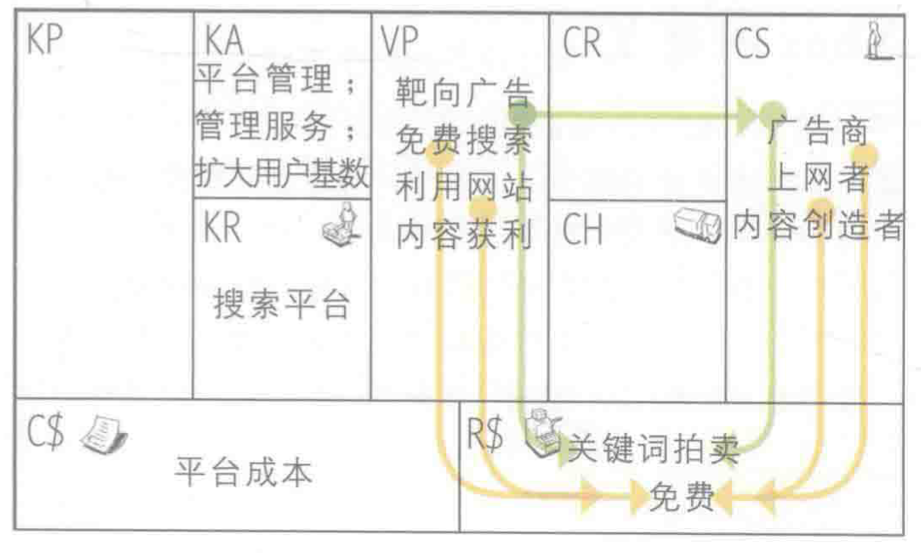
\includegraphics[width=0.65\textwidth]{img/谷歌的商业模式.png}
        \vspace{-0.5em}
	\end{figure}

    \subsubsection{苹果公司的平台运营商进化记}

    \begin{figure}[H]
		\centering
        \vspace{-0.5em}
		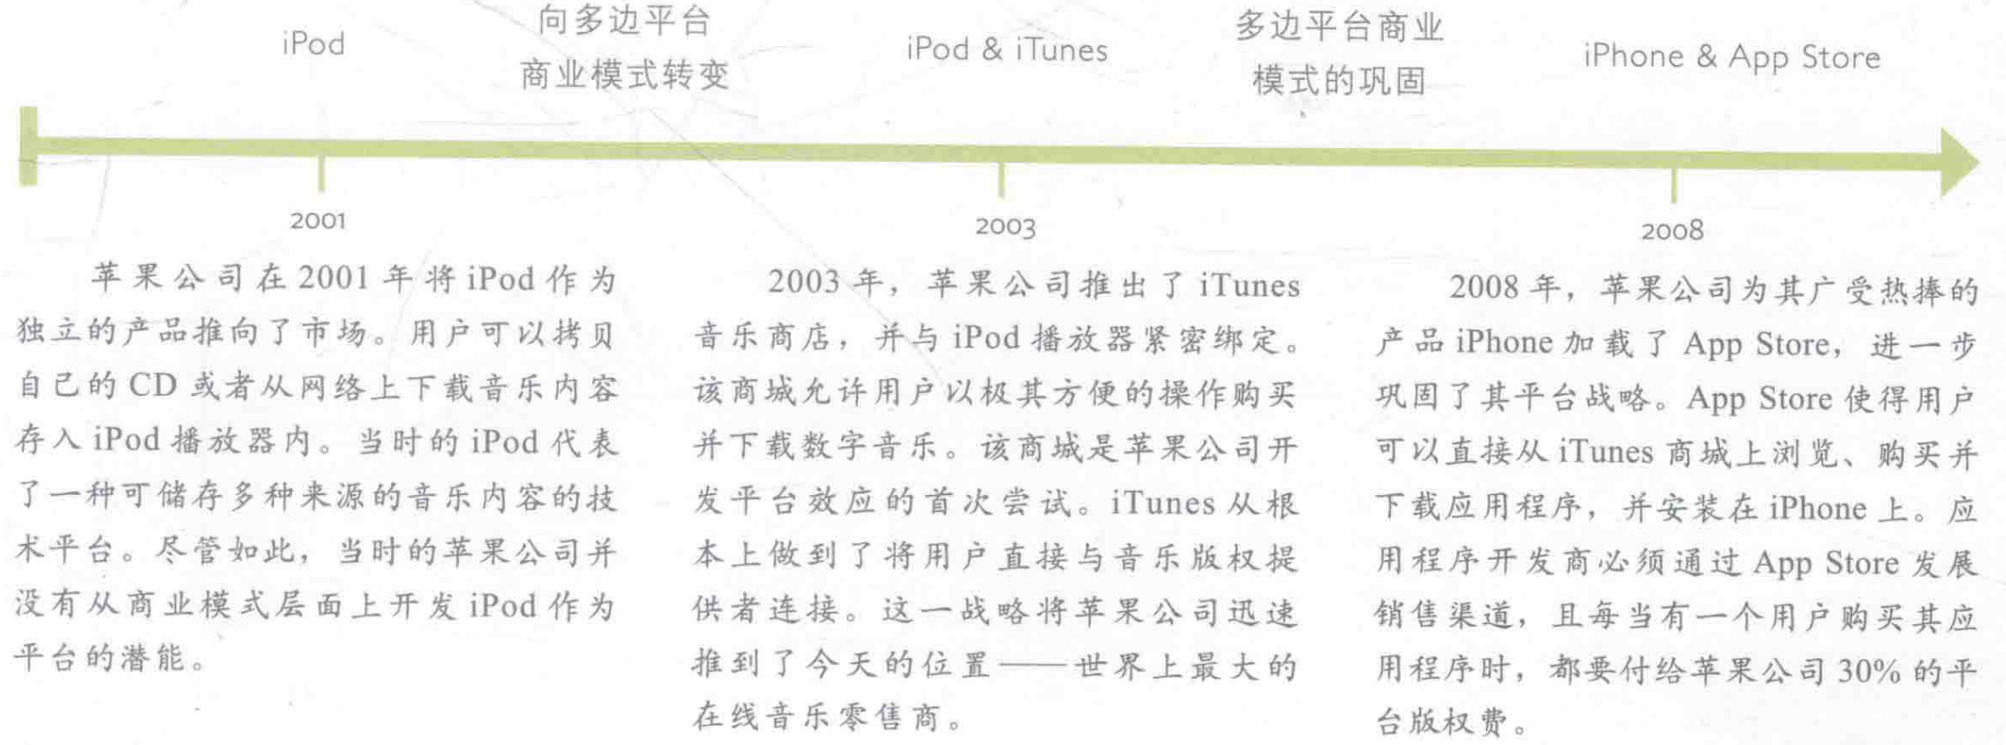
\includegraphics[width=0.95\textwidth]{img/苹果公司的平台运营商进化记.png}
        \vspace{-0.5em}
	\end{figure}

    \subsubsection{多边平台商业模式总结}

    \begin{figure}[H]
		\centering
        \vspace{-0.5em}
		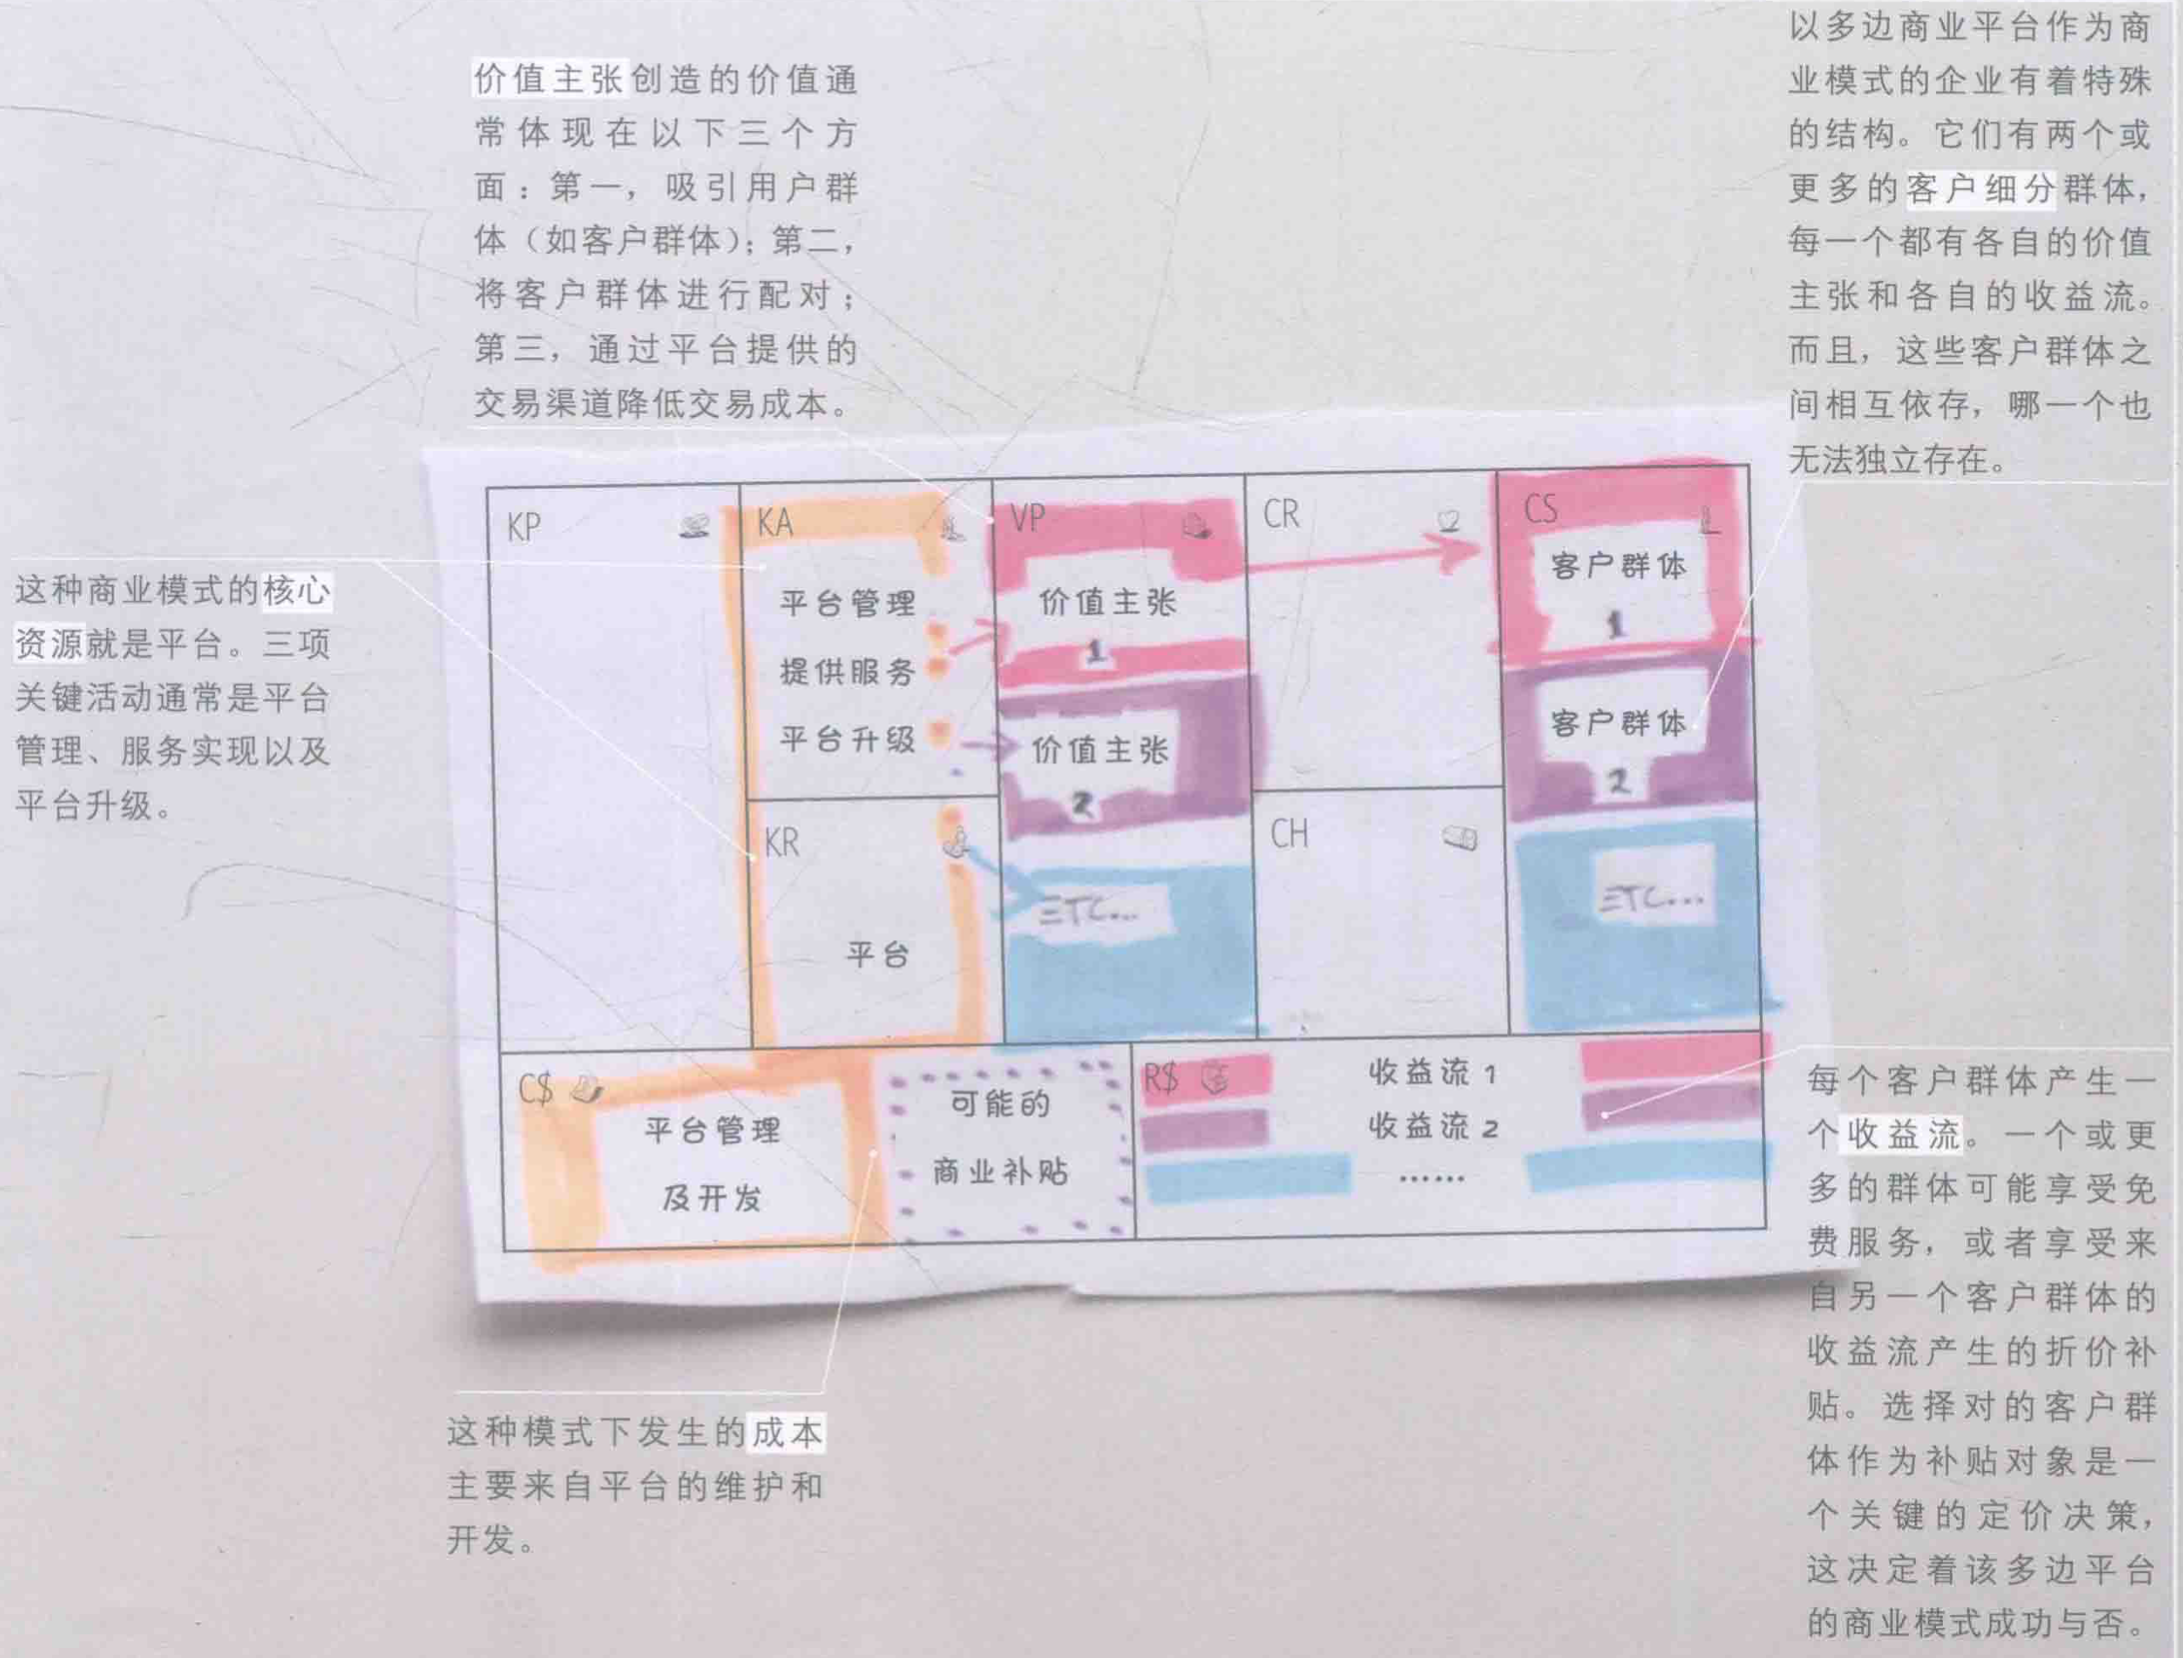
\includegraphics[width=0.95\textwidth]{img/多边平台商业模式总结.png}
        \vspace{-0.5em}
	\end{figure}

    \subsection{免费商业模式}
    在免费商业模式中,至少有一个关键的客户群体是可以持续免费地享受服务
    \begin{itemize}
        \item 不付费的客户所得到的财务支持来自商业模式中的另一个客户群体。
        \item 任何价格为0的产品产生的需求要数倍于价格为1分钱或者其他定价的商品产生的需求。
        \item 数字产品与服务的复制传播成本接近于0,海量用户下边界成本也趋向于0
        \item 三种可行的免费商业模式:
        \begin{itemize}
            \item 广告模式:基于多边平台的免费商品
            \item 免费增值:免费的基本服务,可选的增值服务
            \item 钓鱼模式:以免费或很便宜的初始价格吸引客户,并引导其重复购买
        \end{itemize}
    \end{itemize}

    \subsubsection{广告:一个多边平台商业模式}
    广告是一种实现免费供给的、成熟的收益来源

    这种模式中一个让人印象深刻的例子就是Metro,其天才之处在于改变了传统日报的发行模式
    \begin{itemize}
        \item 它的报纸是免费提供的,派发以在人流密集的办公区以及公共交通网点人工发放或陈列在展架上供行人自取
        \item 它的报纸编辑质量只需要满足年轻的上班族通勤往返途中消磨时间用即可,这就削减了报纸的编辑成本 
    \end{itemize}

    \begin{figure}[H]
		\centering
        \vspace{-0.5em}
		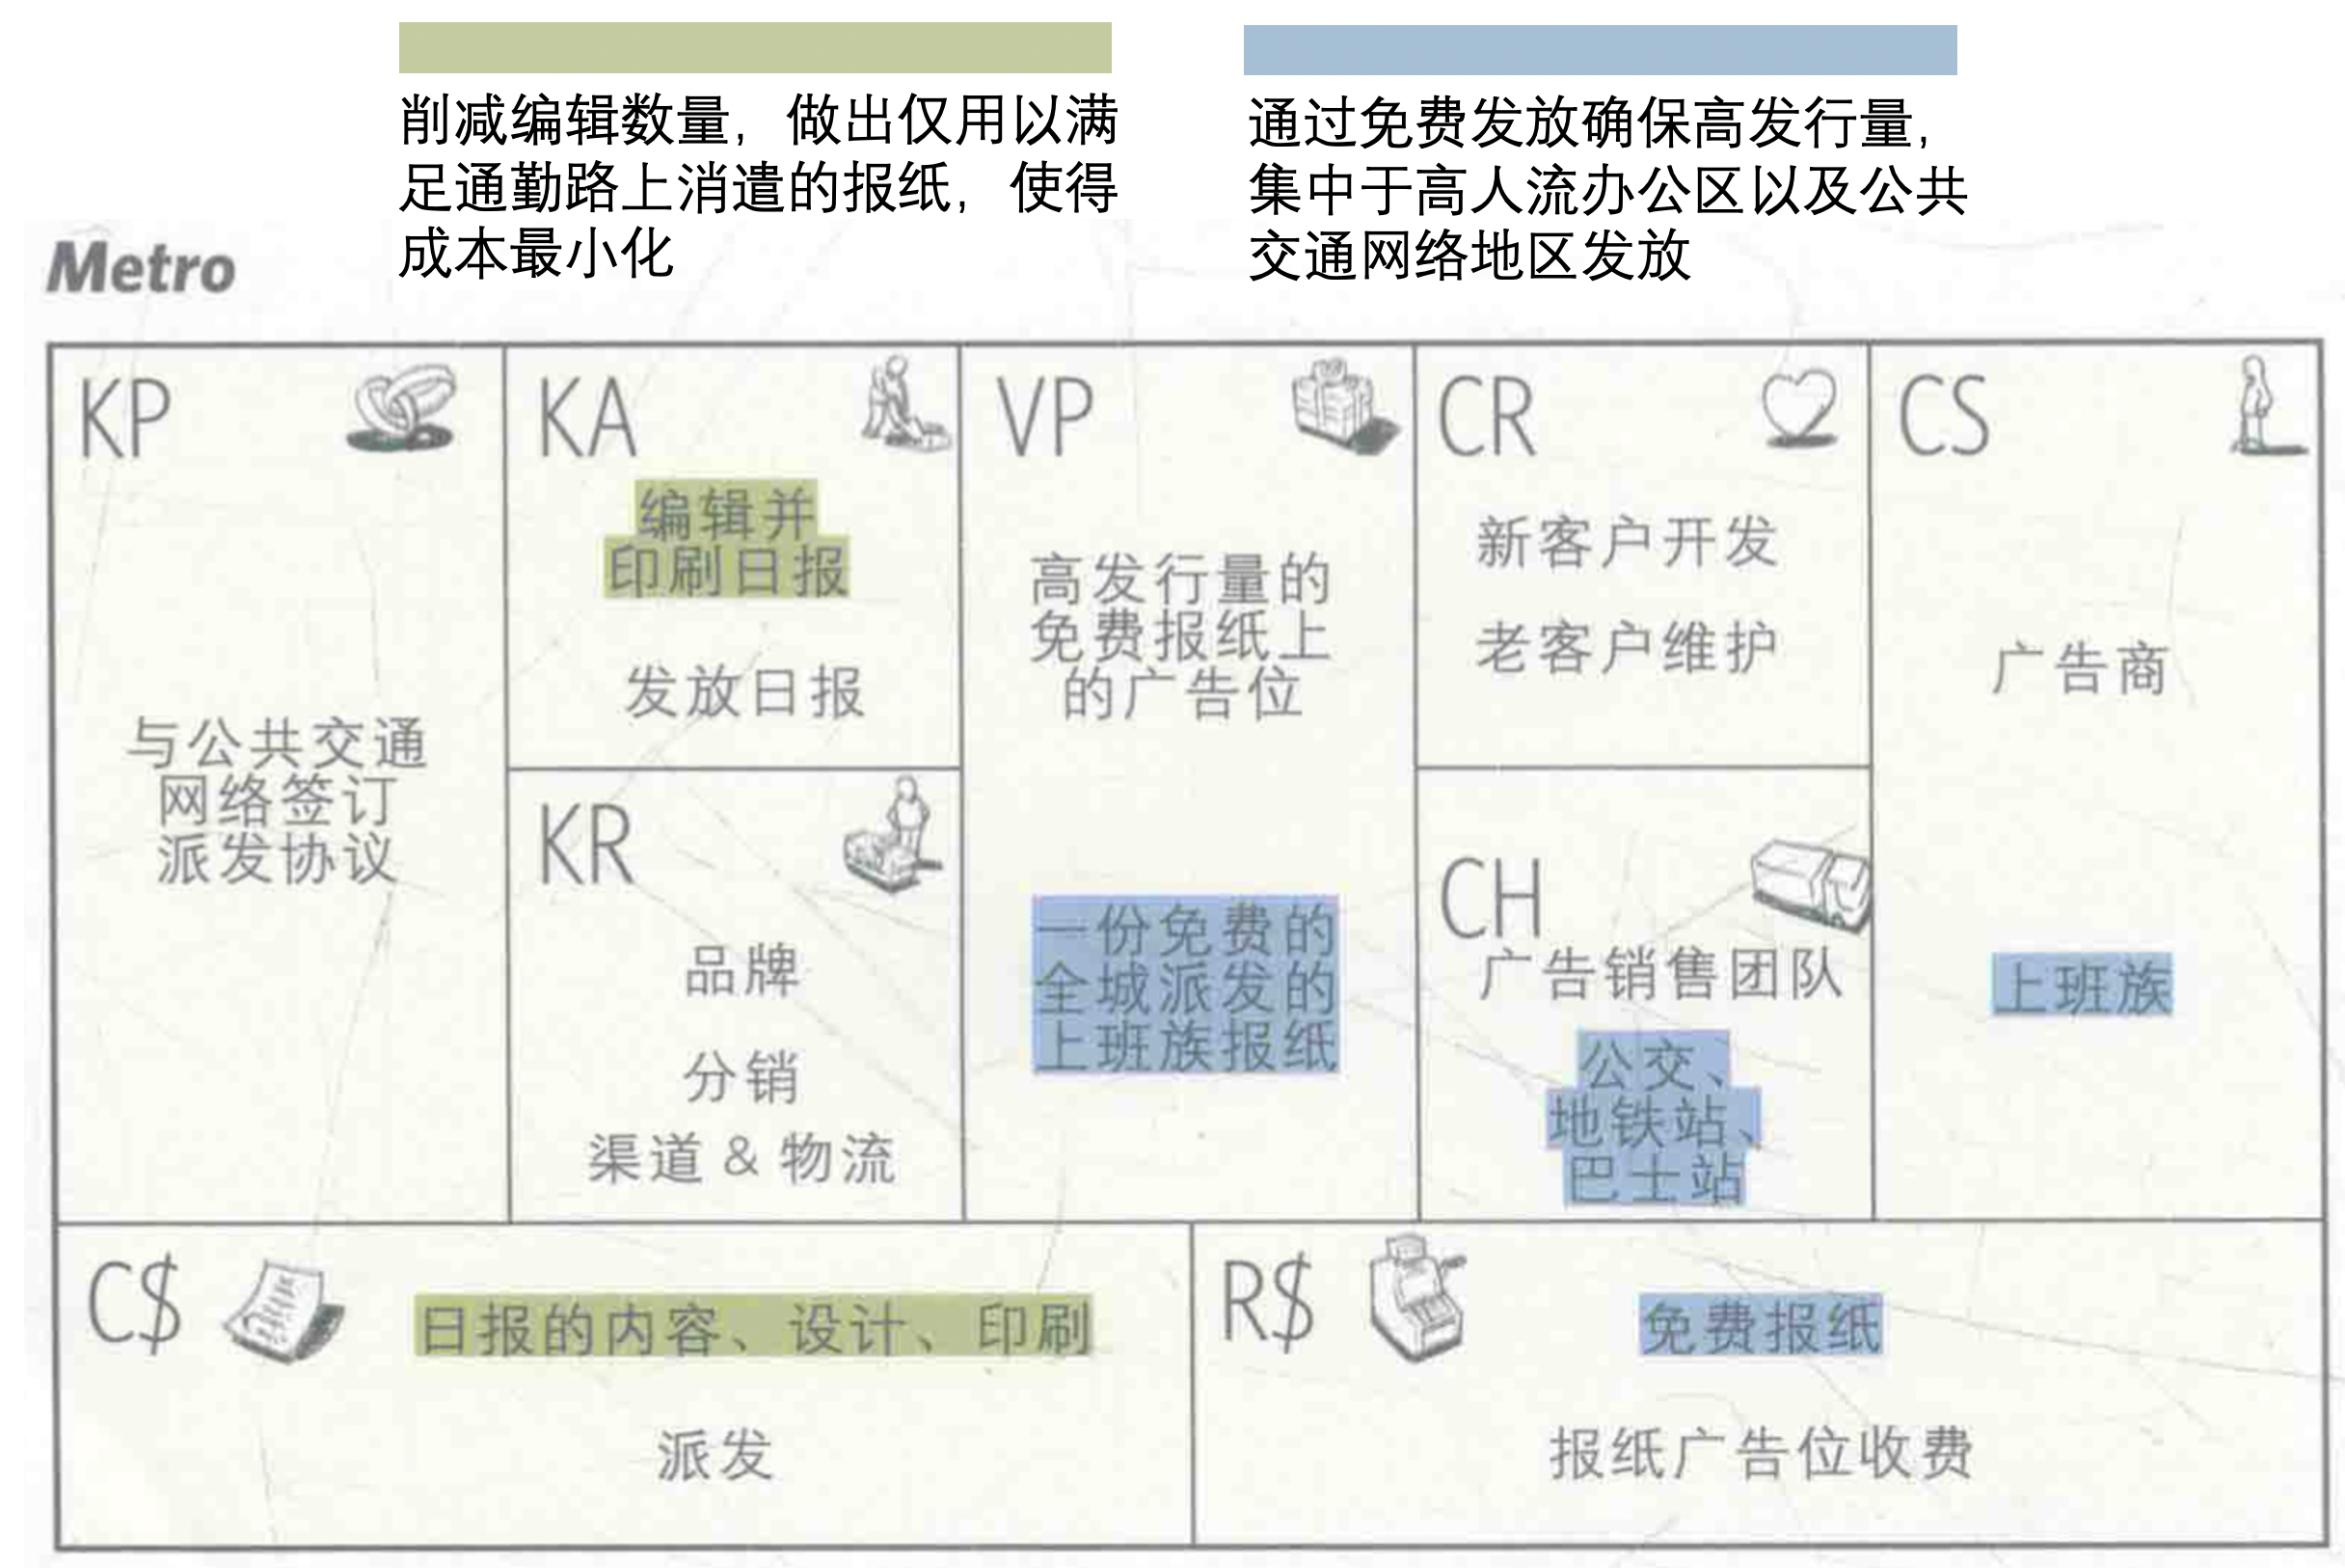
\includegraphics[width=0.7\textwidth]{img/Metro的商业模式.png}
        \vspace{-0.5em}
	\end{figure}

    \begin{figure}[H]
		\centering
        \vspace{-0.5em}
		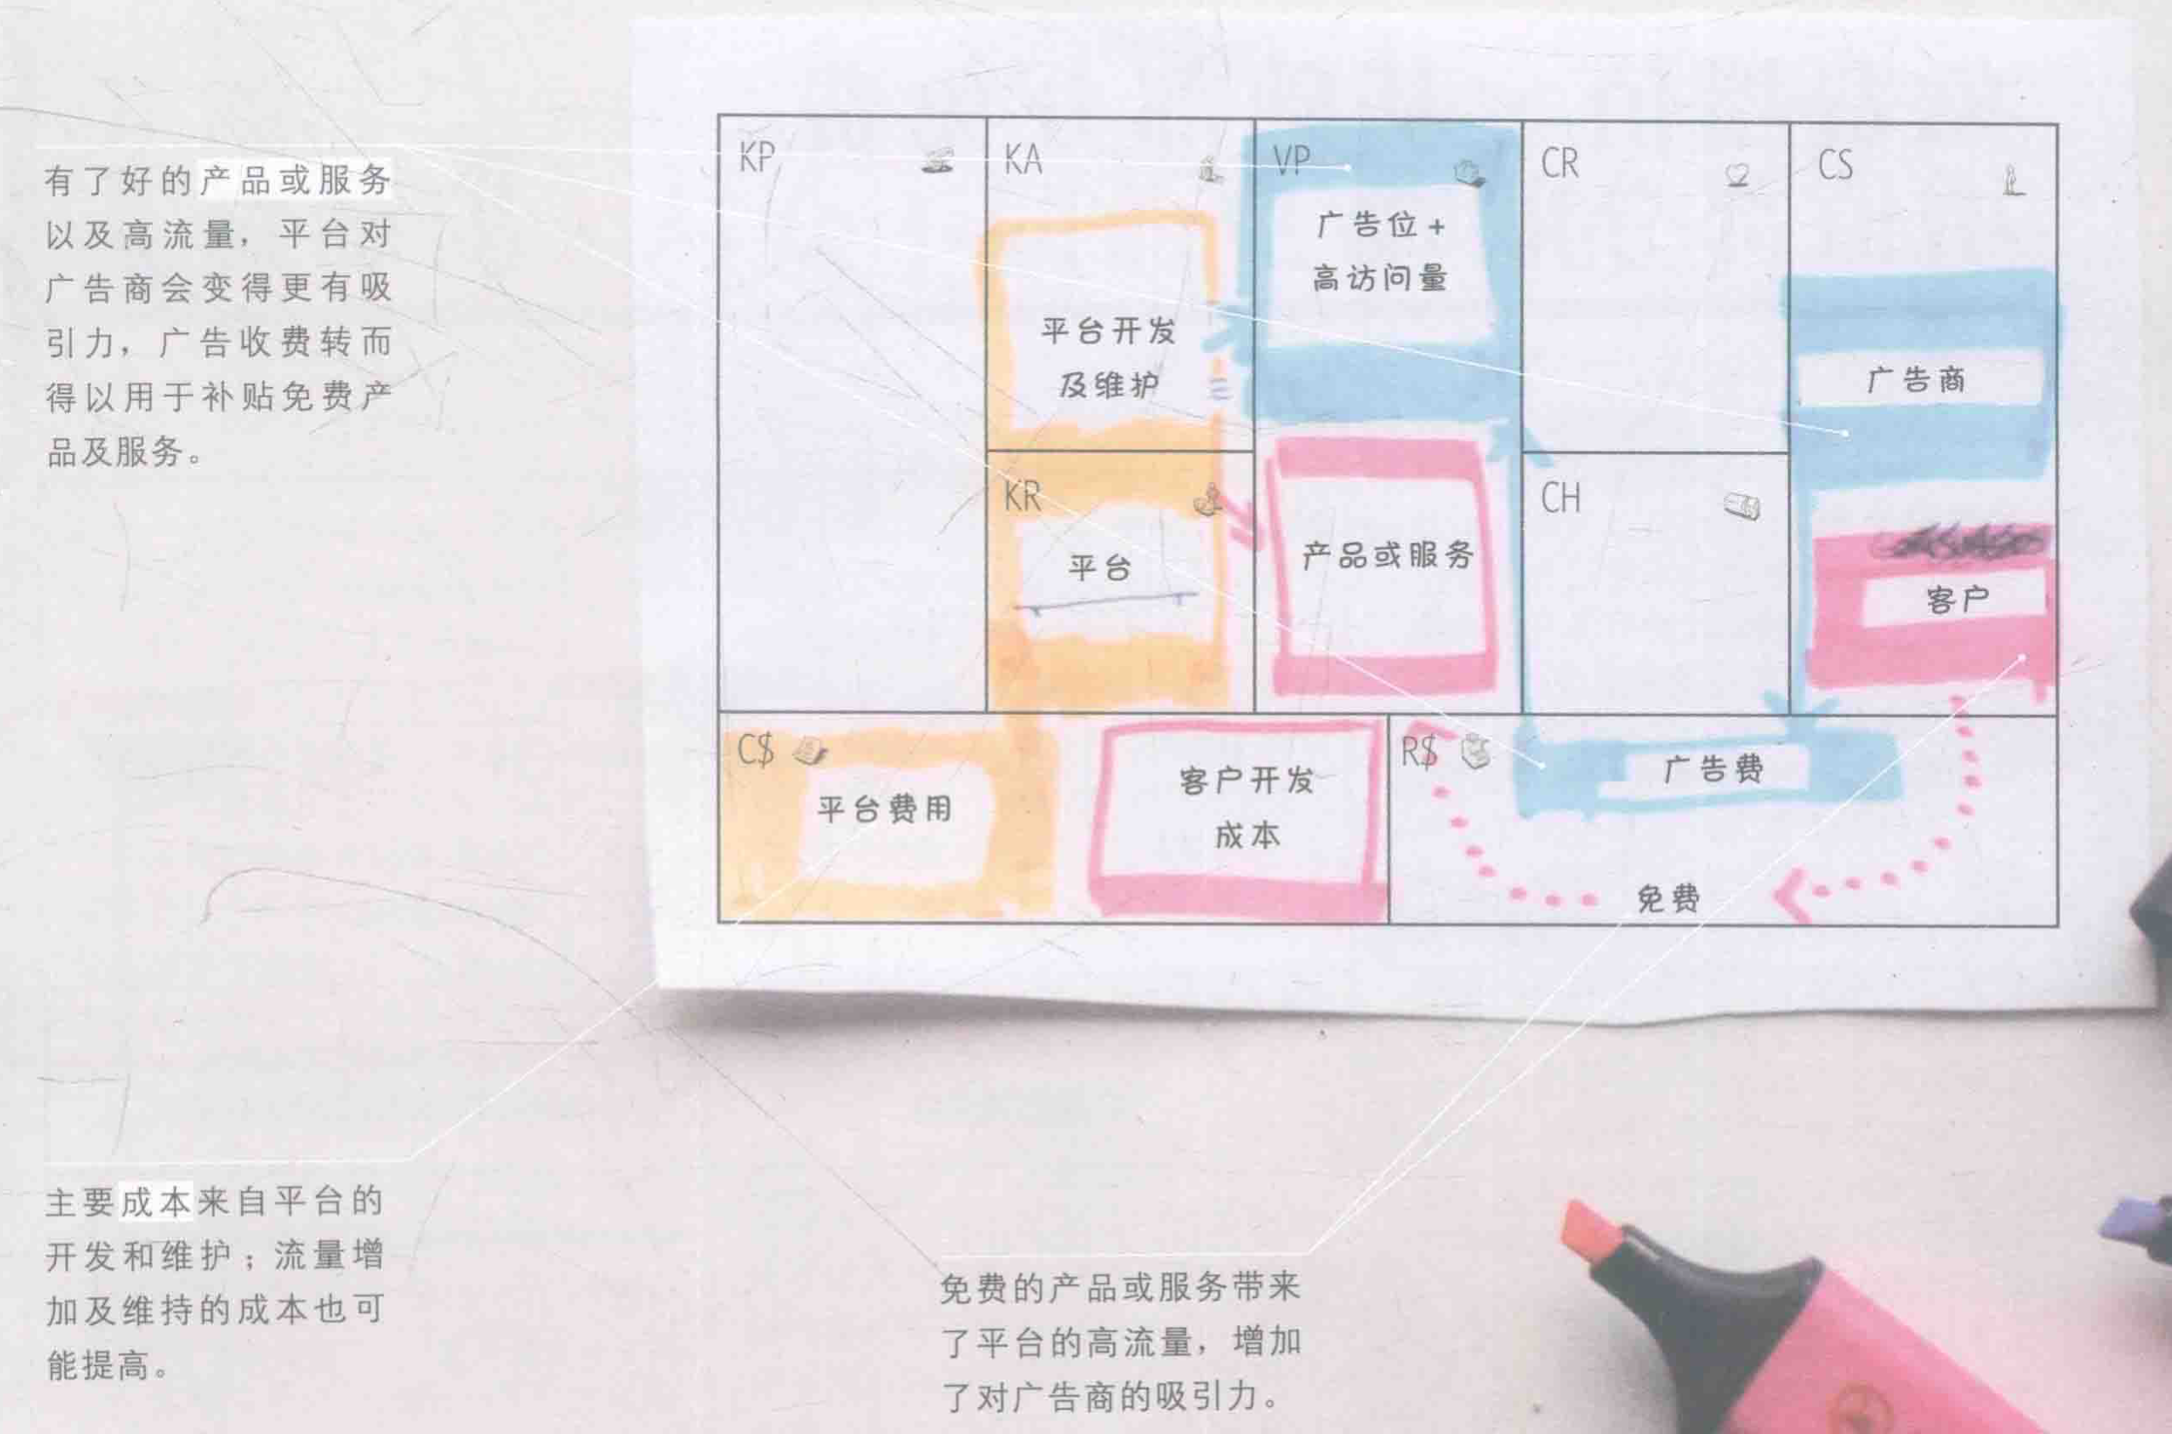
\includegraphics[width=0.8\textwidth]{img/广告:一个多边平台商业模式.png}
        \vspace{-0.5em}
	\end{figure}

    \subsubsection{免费增值:基础部分免费,增值部分收费}
    基于网络将免费的基础服务与付费的增值服务相结合,大量用户从免费服务获益,少量用户为增值服务付费
    \begin{itemize}
        \item 不到10\%的用户会为增值服务付费
        \item 两个关键指标:关注免费用户服务成本(低边界成本)与增值用户转化率
    \end{itemize}

    \paragraph{照片分享网站Flickr}~{}

    Flickr的用户可以免费获得一个基本账户,使得他们得以上传和分享照片。
    \begin{itemize}
        \item 免费服务有一些限制条件,例如有限存储空间以及每月可上传的图片数量有限
        \item 但支付少量的年费,用户就可以买到一个“专业”账户,并享受无限量的上传数量和存储空间,以及一些额外功能
    \end{itemize}
    \begin{figure}[H]
		\centering
        \vspace{-0.5em}
		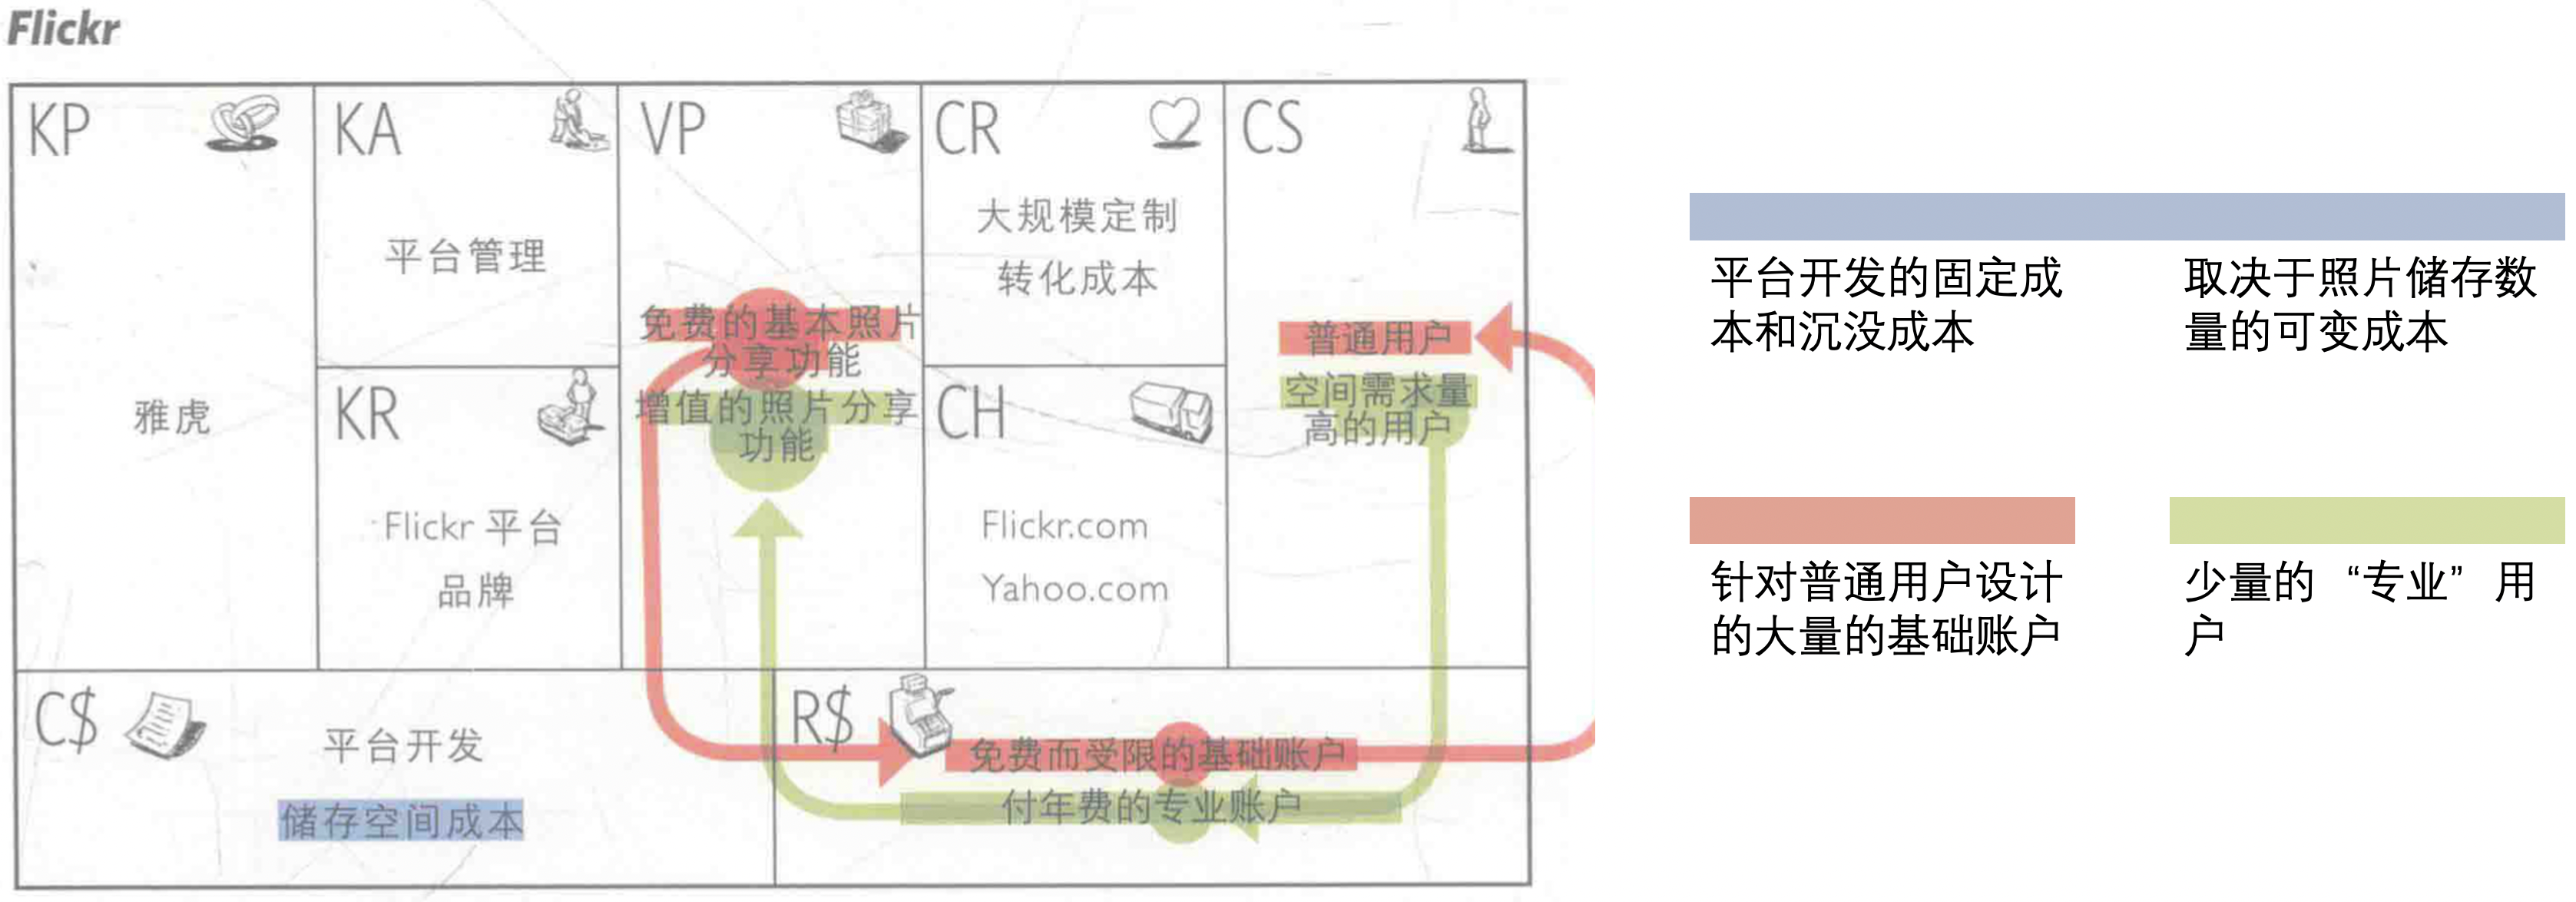
\includegraphics[width=0.98\textwidth]{img/Flicker的商业模式.png}
        \vspace{-0.5em}
	\end{figure}

    \paragraph{开放源码:与众不同的免费增值}~{}

    红帽公司(RedHat)将产品建立在开放源码的方式上。红帽公司明白,企业对耐用又免使用许可费的开放软件源码感兴趣,但因为没有任何实体对这些源码负责并提供维护而不愿使用它们。红帽公司填补了这个缺口,它免费提供稳定的、通过测试的、完整可使用的开放软件源码。
    \begin{itemize}
        \item 代码免费完整开放(多种许可证)
        \item 年费换取最新源码使用权、无限制服务支持、产品法律上拥有者联系的保证    
    \end{itemize}
    \begin{figure}[H]
		\centering
        \vspace{-0.5em}
		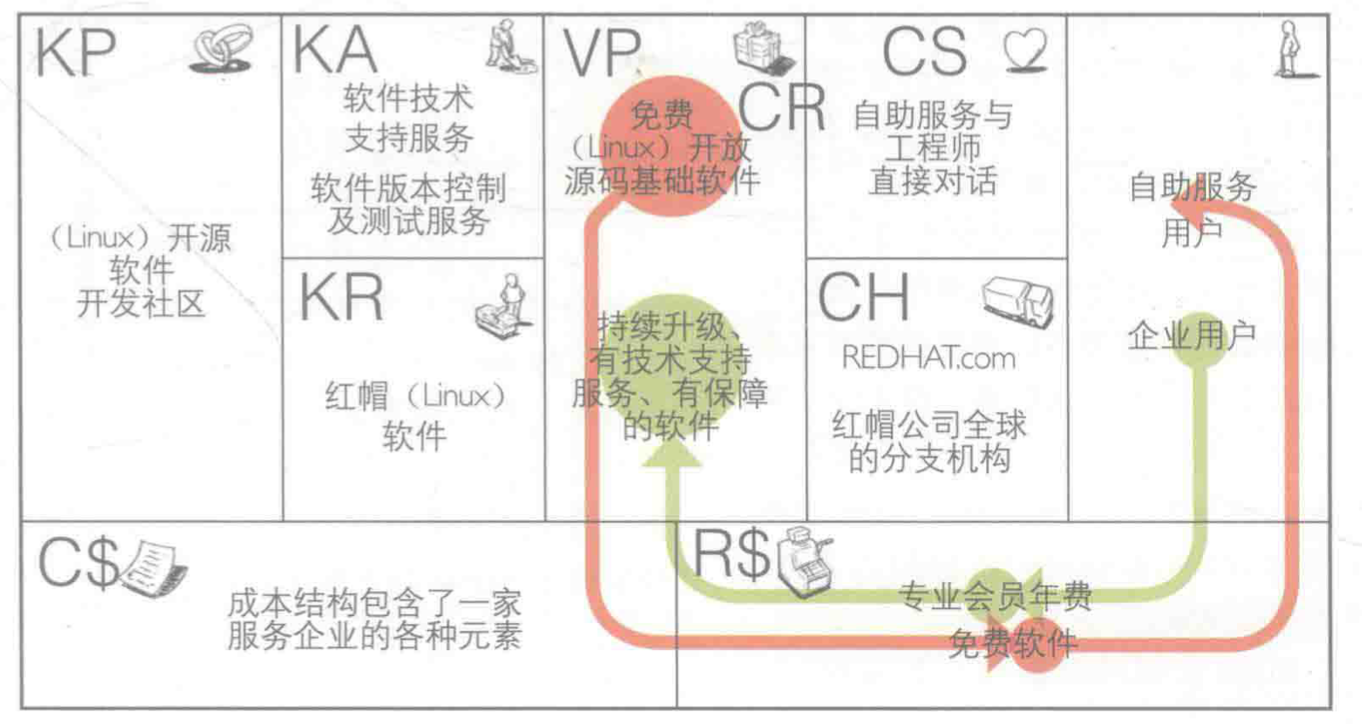
\includegraphics[width=0.7\textwidth]{img/RedHat的商业模式.png}
        \vspace{-0.5em}
	\end{figure}

    \paragraph{Skype的商业模式}~{}


    \begin{figure}[H]
		\centering
        \vspace{-0.5em}
		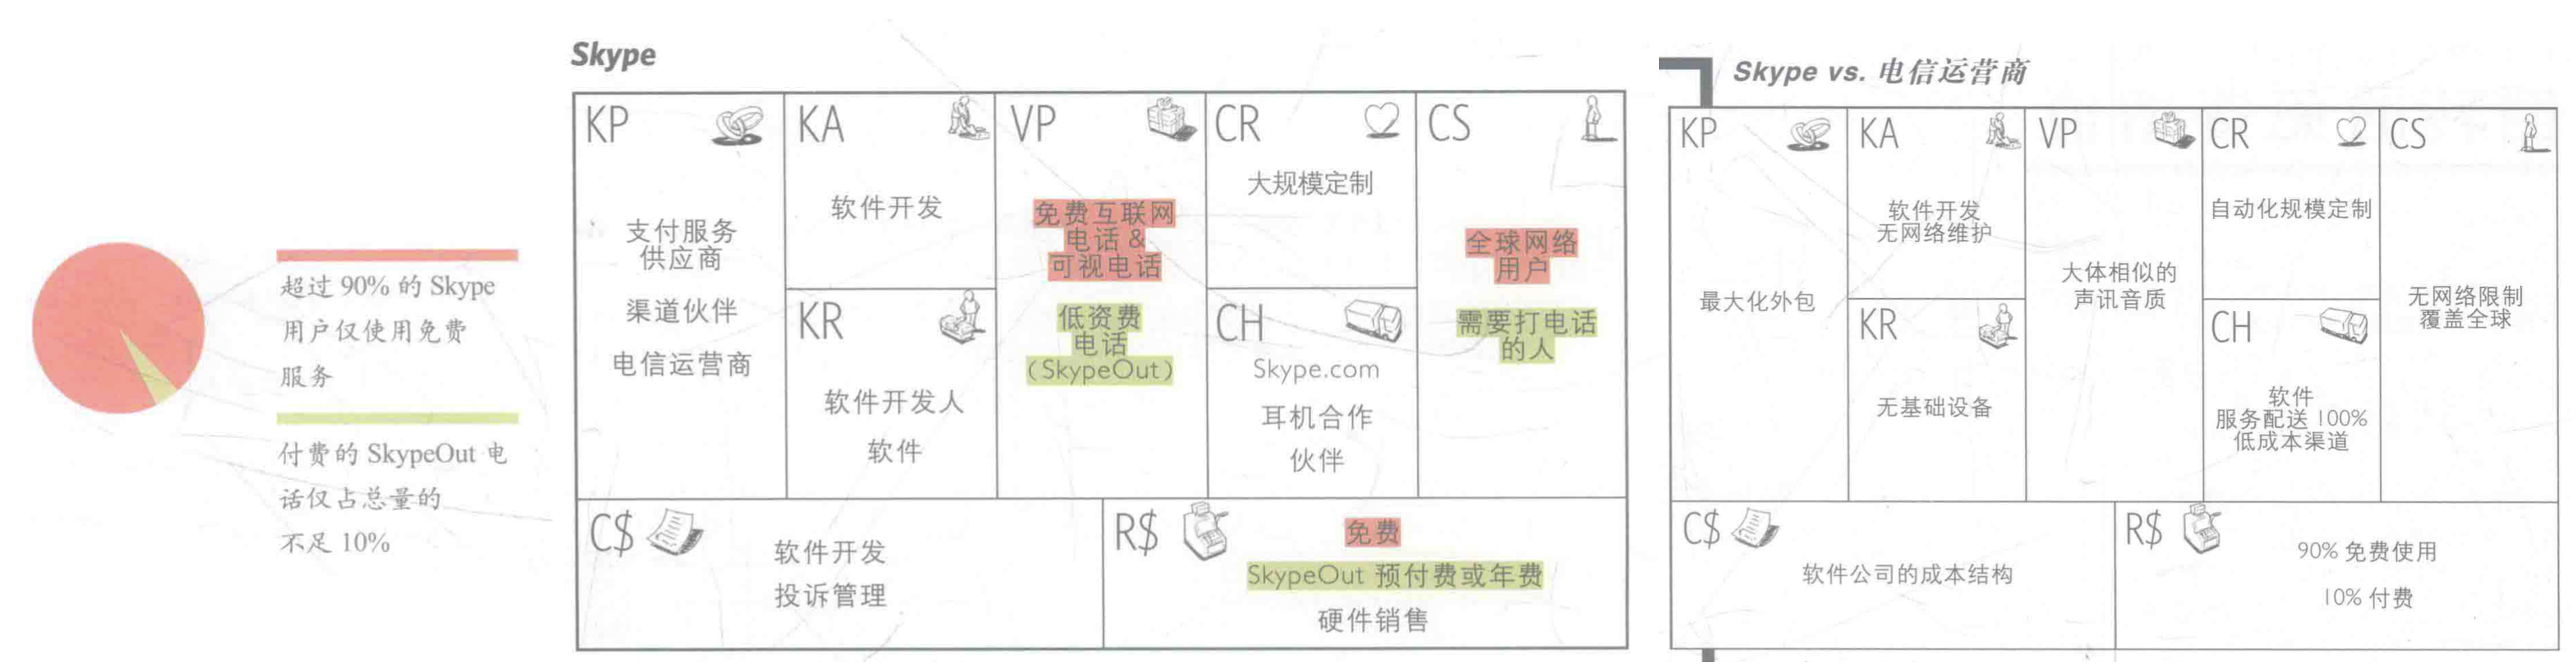
\includegraphics[width=\textwidth]{img/Skype的商业模式.png}
        \vspace{-0.5em}
	\end{figure}

    Skype以网络实现免费通话服务,对电信行业造成了破坏
    \begin{itemize}
        \item Skype公司开发了同名软件,可以安装于电脑或智能手机上,帮助用户之间实现设备间的免费通话
        \item Skype之所以能做到这一点是因为它的成本结构完全不同于电信运营商。免费电话的实现方式是路由互联网,基于对等计算技术,将用户的硬件设备和互联网当作通信的基础设备。因此,Skype不需要像电信运营商那样管理一套自有的网络设备,而只需要为每一位增加的用户支付少量的成本
        \item 用户只有在拨打固定电话的时候才需要付费,移动电话则通过一项叫作SkvpeOut的增值服务以非常低的费率享受与固定电话的通话服务
    \end{itemize}


    \paragraph{保险行业模式:倒转的免费增值}~{}

    在保险行业模式中,由大部分的客户定期支付小额保费以确保自己手虽不易发生却可能带来经济上的灾难的事件。简而言之,是大部分的付费客户来补贴那一小部分产生实际保险索赔的客户,但是任何一个付费客户都有可能随时变成受益群体中的一员。

    REGA是瑞士的一家非营利机构,它使用直升机和飞机将医护人员送到事故发生地点,这在多山的瑞士作用尤其显著。该组织有超过200万名“捐赠者”资助。作为回报,捐赠人免费享受REGA的一切救助。山间救援操作大多十分昂贵,因此REGA的捐赠者认为这样的服务十分有吸引力,可以帮助他们规避在滑雪假期、夏日徒步或者山间驾驶过程中,因可能发生的意外而支付高昂的救援花费。
    \begin{figure}[H]
		\centering
        \vspace{-0.5em}
		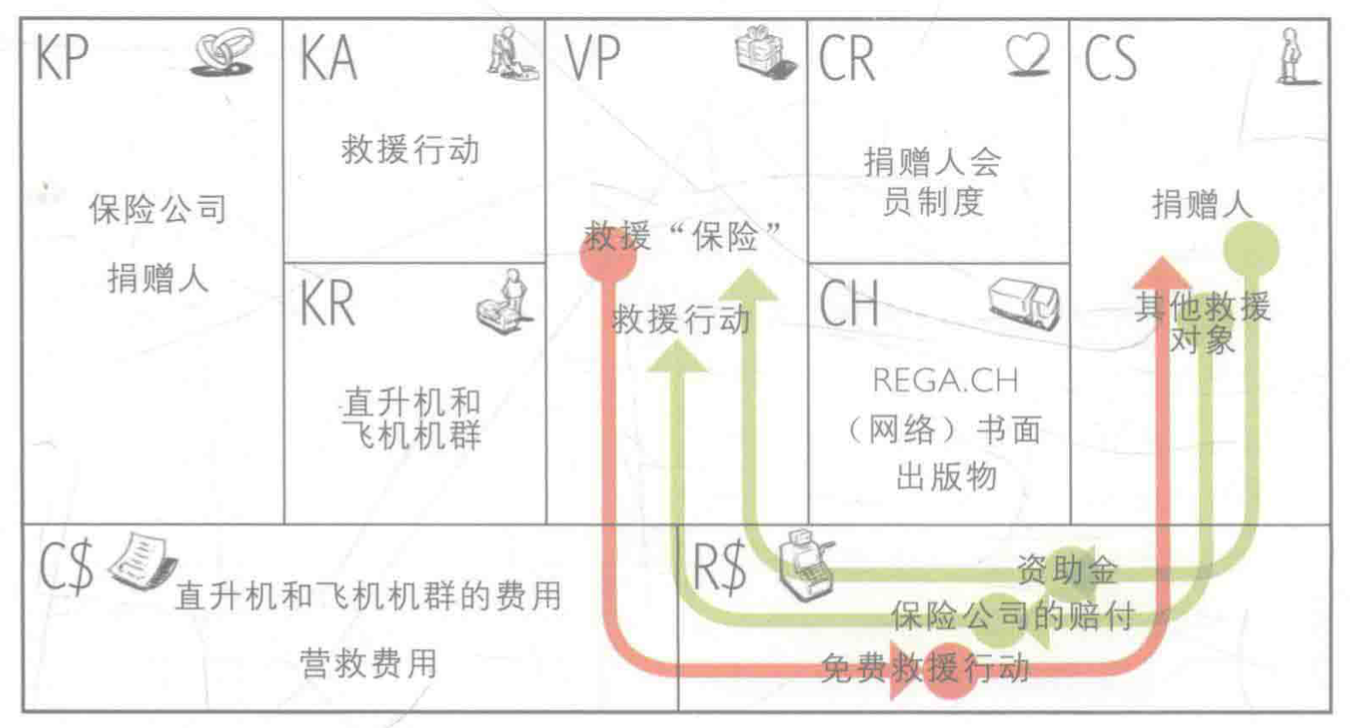
\includegraphics[width=0.7\textwidth]{img/保险行业模式.png}
        \vspace{-0.5em}
	\end{figure}

    \paragraph{免费增值模式总结}~{}

    \begin{itemize}
        \item 平台是免费增值模式最重要的资产,因为它使得免费的基础服务以低边际成本实现
        \item 客户关系是自动的且低成本的,因为有大量的免费用户数量
        \item 免费用户向增值用户的转化率,是一个很重要的衡量指标
        \item 该模式的成本结构分为三部分:可观的固定成本,为免费账户提供的低边际成本服务,以及(独立的)增值账户成本
        \begin{itemize}
            \item 收入 $=$ 用户数量 $\times$ 增值用户比重 $\times$ 增值服务价格 $\times$ 增长率 $\times$ 顾客流失
            \item 服务成本 $=$ 免费用户数 $\times$ 免费服务成本 $+$ 增值用户数 $\times$ 增值服务成
            \item 运营利润 $=$ 收入 $-$ 服务成本 $-$ 固定成本 $-$ 获客成本
        \end{itemize}
    \end{itemize}

    \begin{figure}[H]
		\centering
        \vspace{-0.5em}
		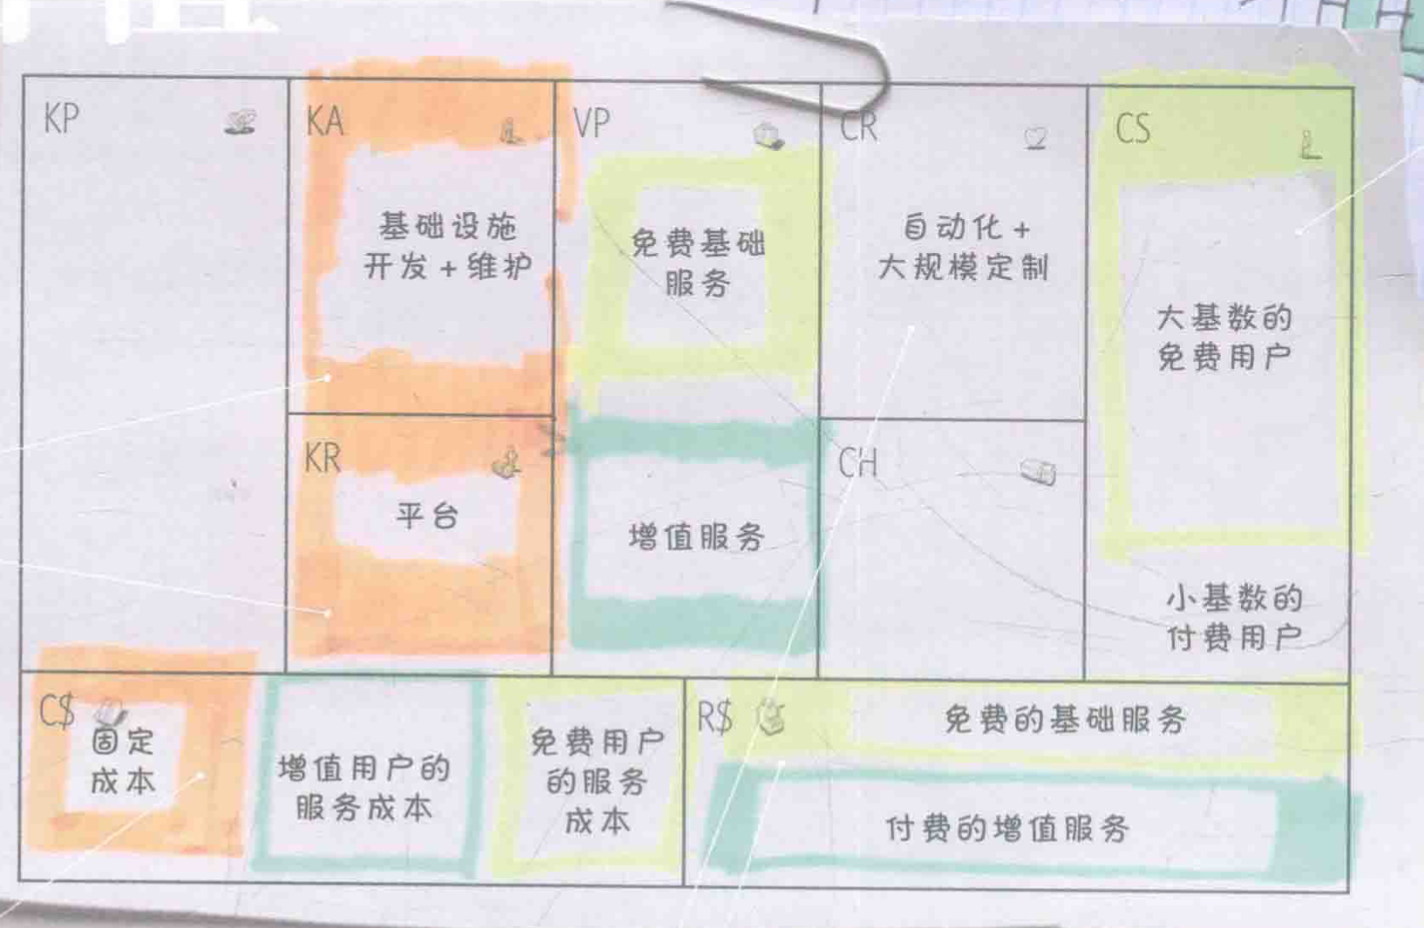
\includegraphics[width=0.7\textwidth]{img/免费增值模式总结.png}
        \vspace{-0.5em}
	\end{figure}

    \subsubsection{诱饵\&陷阱模式}

    诱饵\&陷阱模式的特点是期初以不贵的或者免费的价格提供有吸引力的商品,且该商品还将进一步地鼓励对相关产品或服务的不断消费
    \begin{itemize}
        \item 这一模式也被称作“招徕定价”或者“剃刀\&刀片”模式
        \begin{itemize}
            \item “招徕定价”是指期初以补贴价格,甚至亏本的价格提供商品,意图通过后续消费获得利润
            \item “剃刀\&刀片”模式是指因发明了一次性刀片而风靡的商业模式
        \end{itemize}
        \item 举例:剃刀+一次性刀片,打印机+墨盒/硒鼓,合约机等
    \end{itemize}

    \begin{figure}[H]
		\centering
        \vspace{-0.5em}
		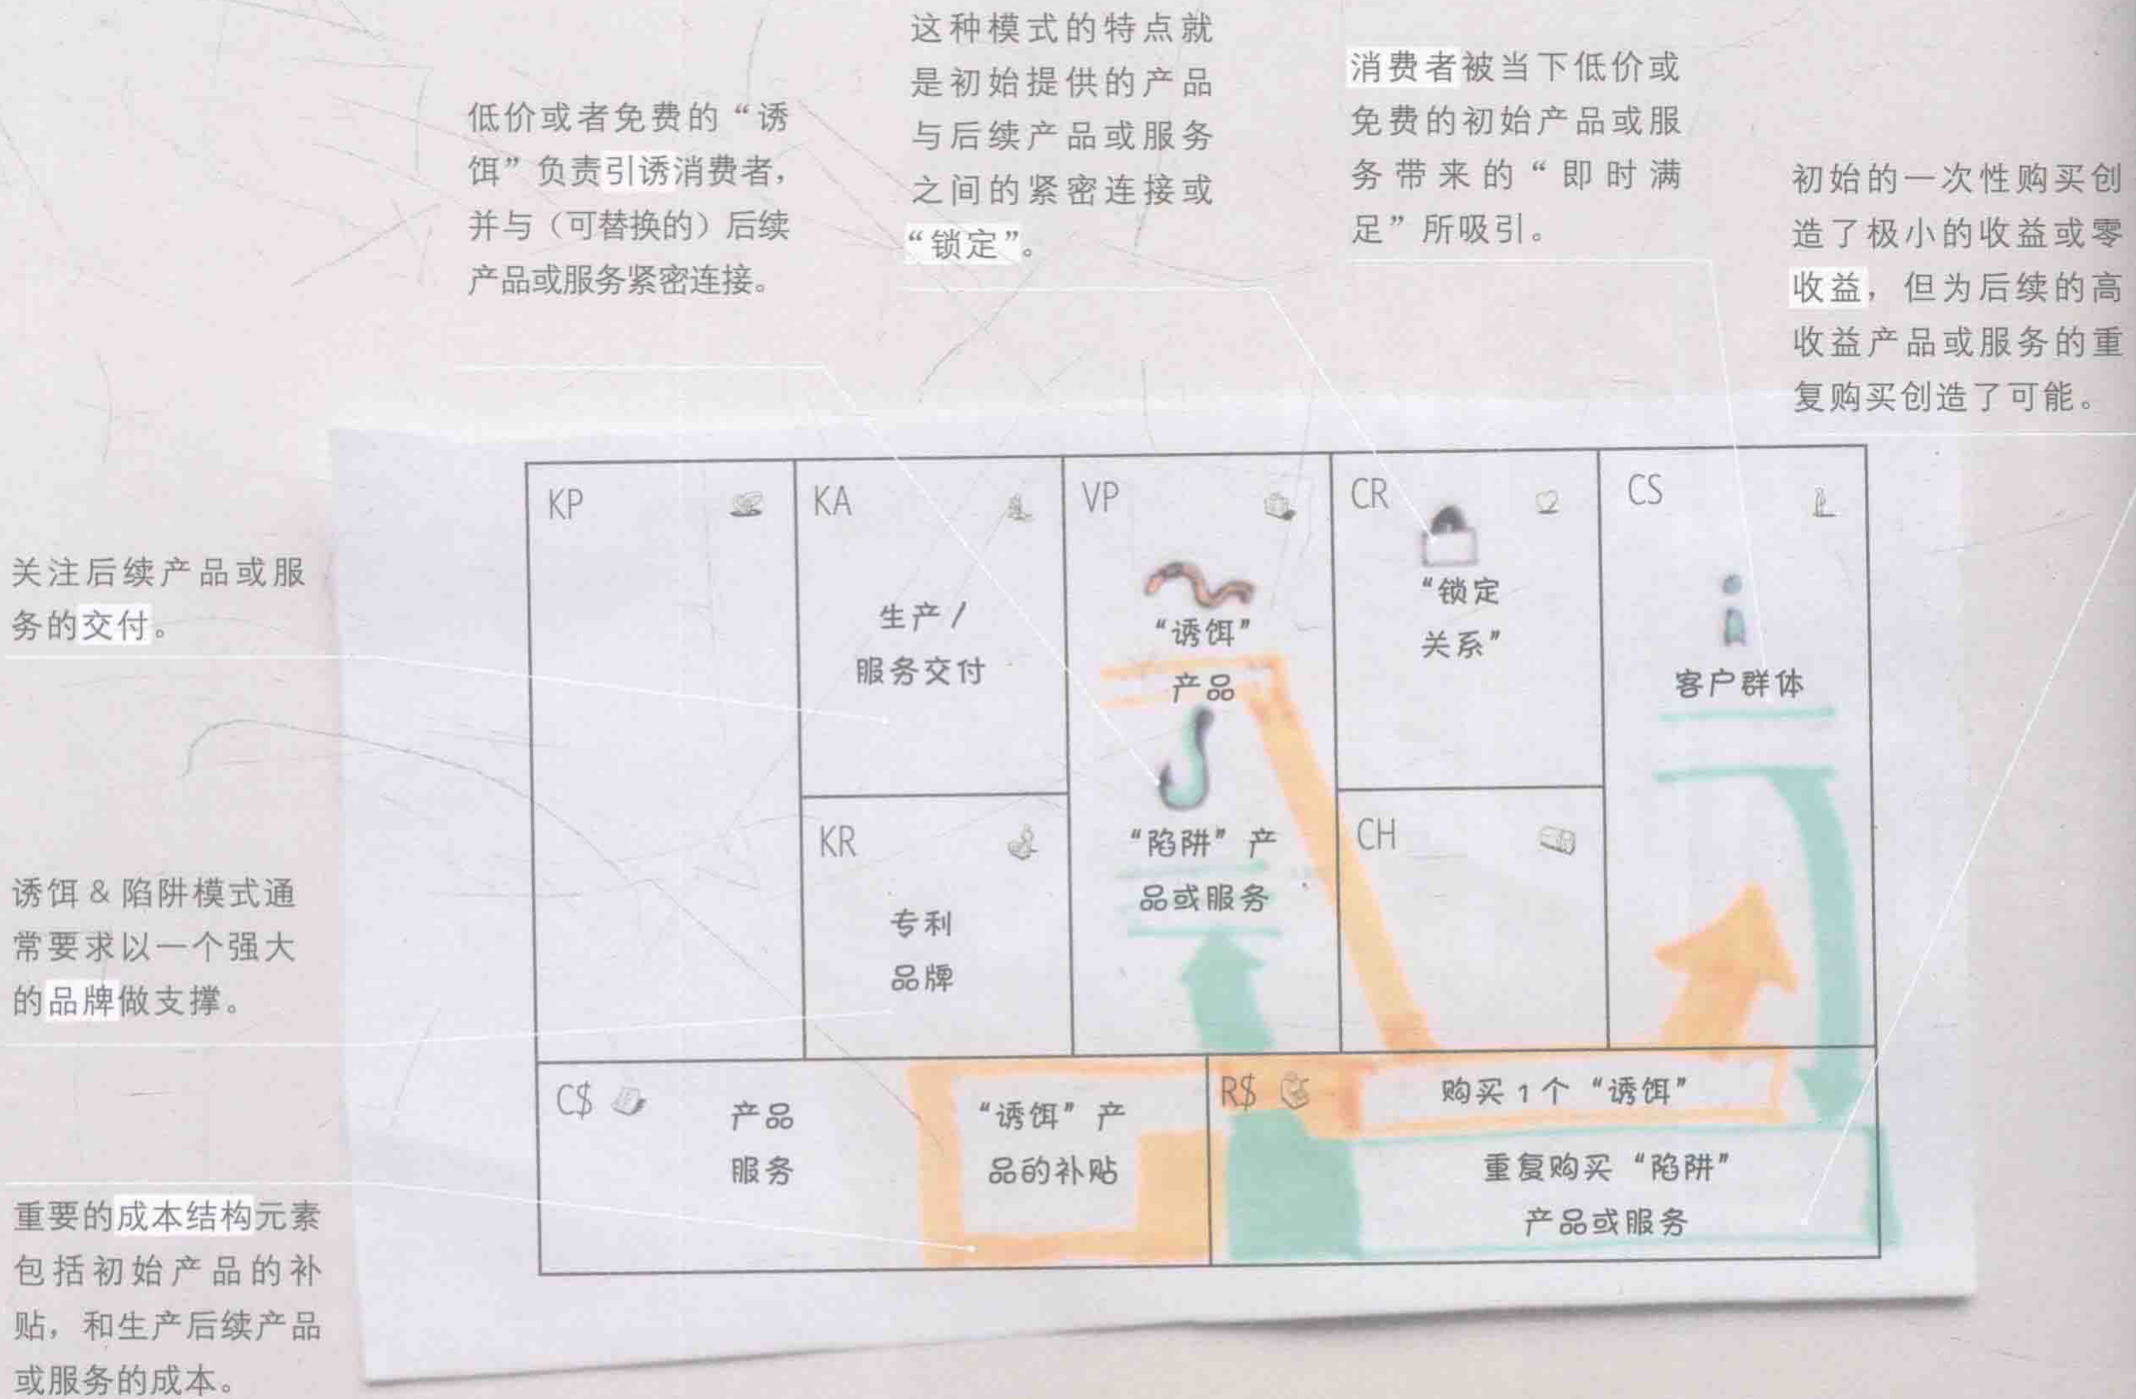
\includegraphics[width=0.8\textwidth]{img/诱饵&陷阱模式.png}
        \vspace{-0.5em}
	\end{figure}

    \subsection{开放式商业模式}
    开放的商业模式适用于通过与外部合作伙伴系统地配合而创造和获取价值的企业。这种模式可以是“由外而内”地于企业内部尝试来自外部的理念,或者“由内而外”地向外部合作伙伴输出公司无用的理念或资产。

    \begin{figure}[H]
		\centering
        \vspace{-0.5em}
		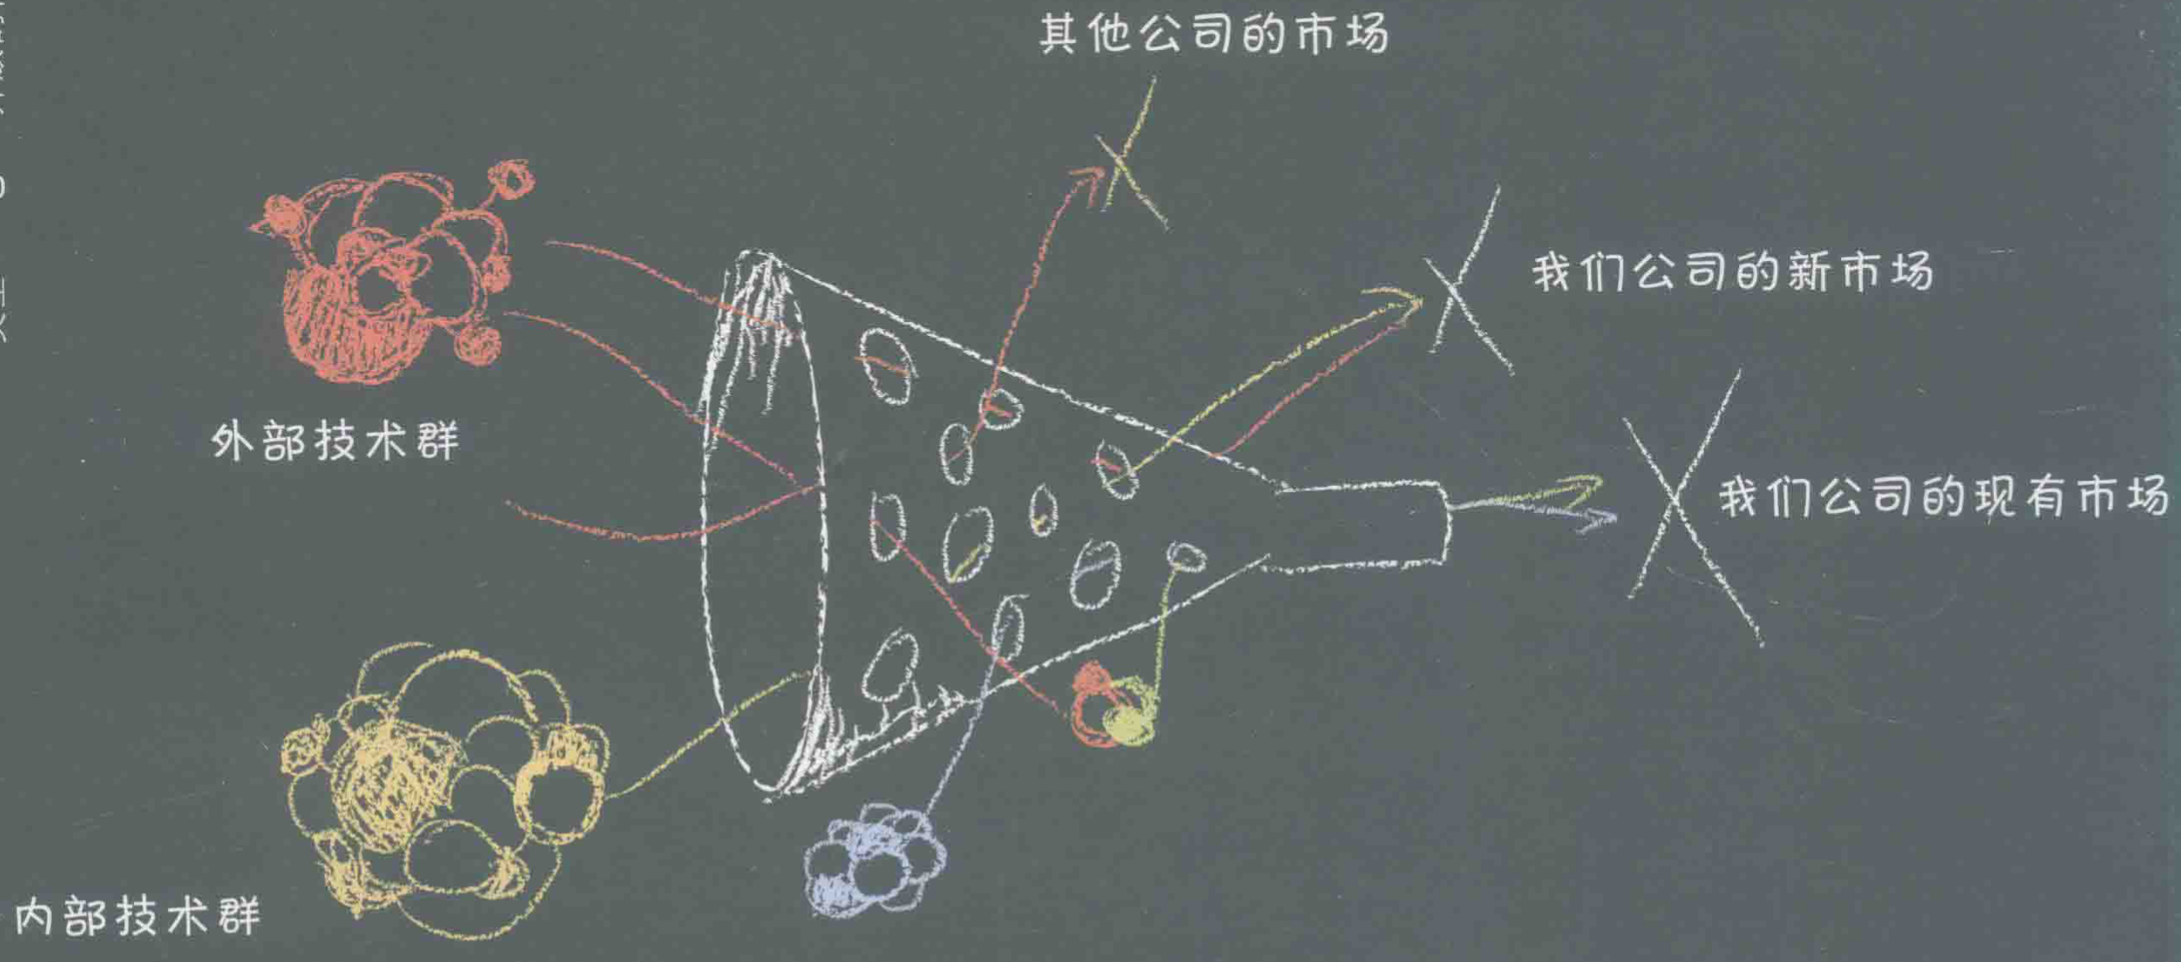
\includegraphics[width=0.55\textwidth]{img/开放的商业模式.png}
        \vspace{-0.5em}
	\end{figure}

    “开放式的创新”和“开放的商业模式”是由亨利·切萨布鲁夫提出的两个术语。它们意指将企业的研发流程向外界敞开
    \begin{itemize}
        \item 切萨布鲁夫主张,在一个以发散的知识为特征的世界中,组织可以通过将外部的知识、知识产权和产品整合进自身的创新流程,进而创造更大的价值并更好地利用自己的研发能力
        \item 此外,切萨布鲁夫演示了,对某家企业而言无用的产品、技术、知识和知识产权可以通过同意许可、合资或者剥离的方式供给外部团体使用,从而变现
        \item 切萨布鲁夫将“由外而内”的创新和“由内而外”的创新区分开来
        \begin{itemize}
            \item “由外而内”的创新发生于当组织将来自外部的理念技术或知识产权引入自身的发展和商业流程
            \item “由内而外”的创新发生于当组织同意许可或出售其知识产权或技术,尤其是闲置资产
        \end{itemize}
    \end{itemize}

    \begin{figure}[H]
		\centering
        \vspace{-0.5em}
		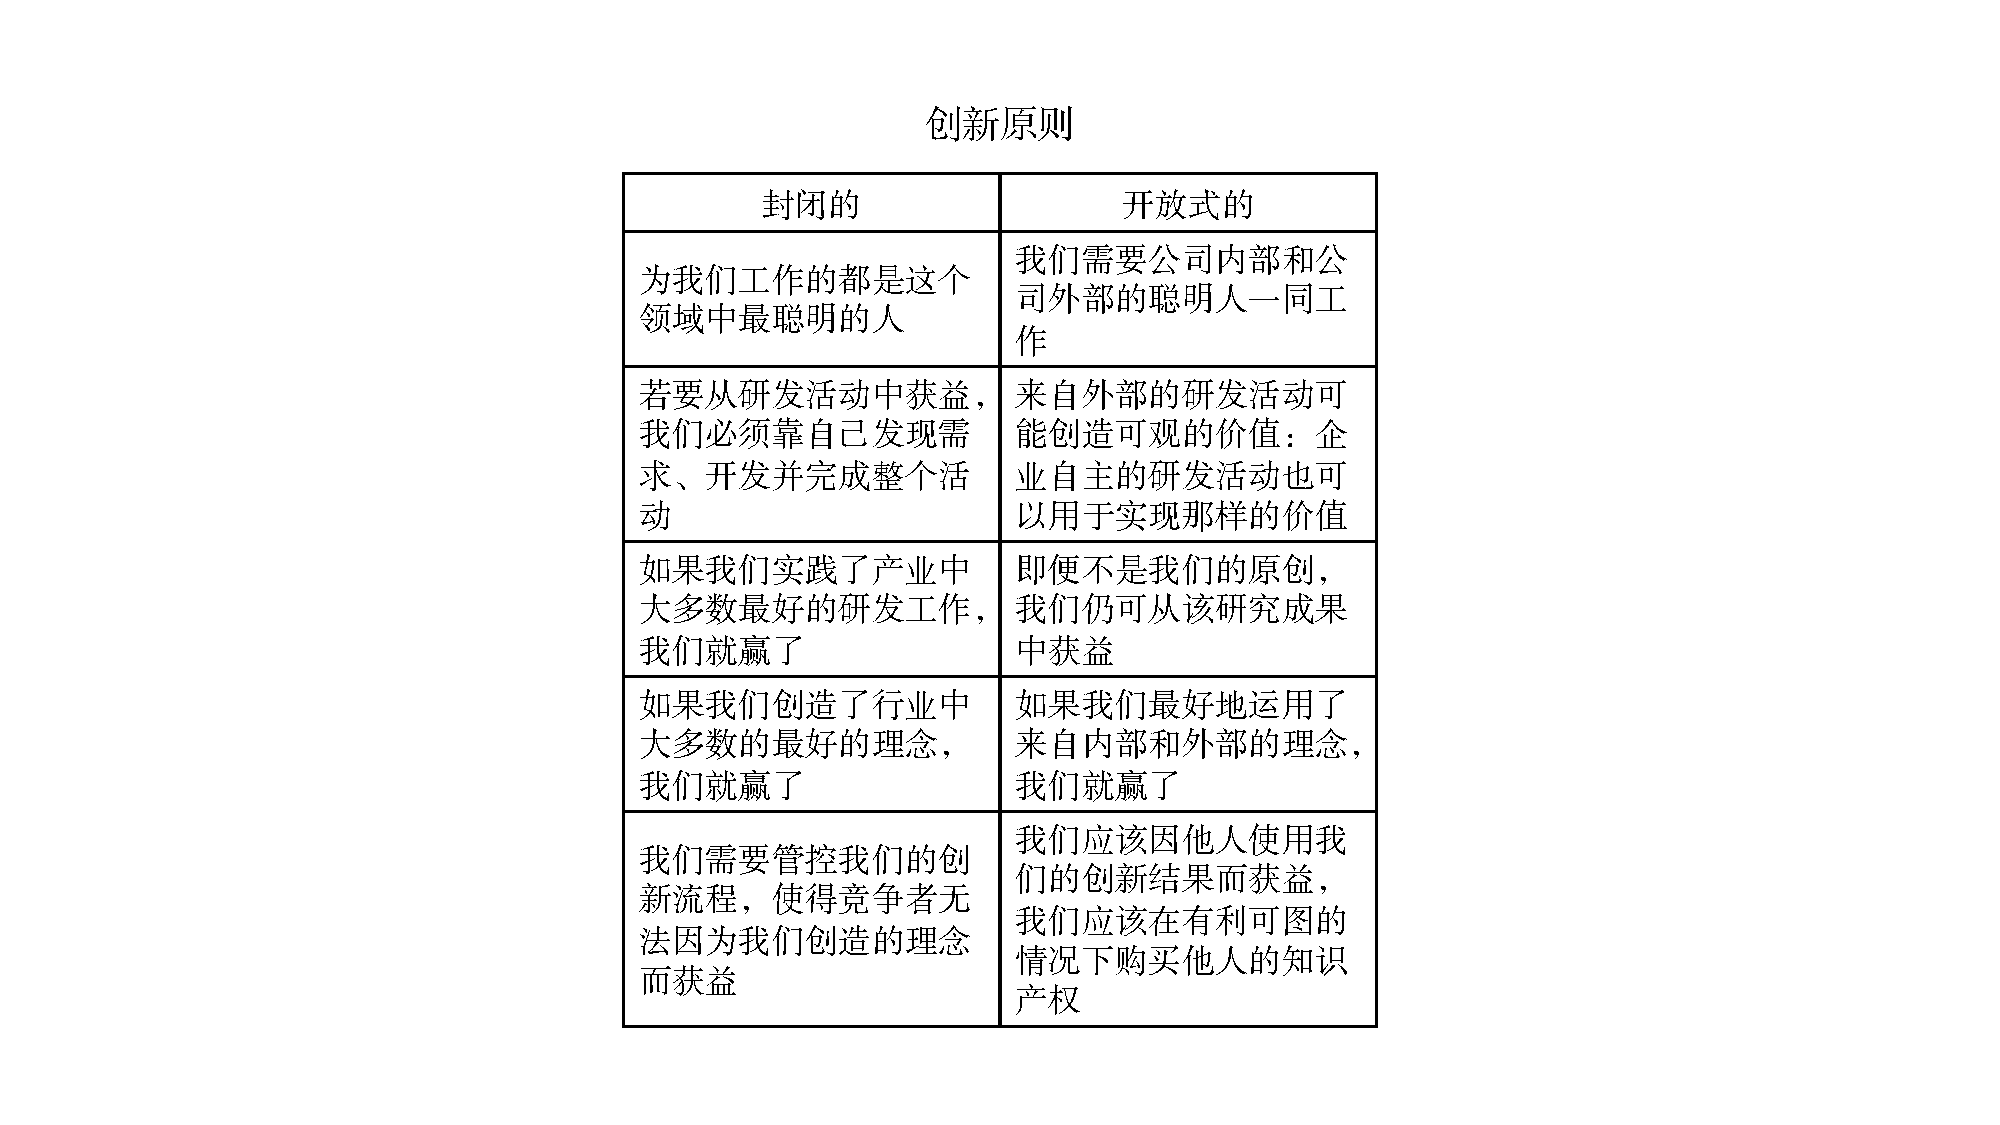
\includegraphics[width=0.4\textwidth]{img/创新原则.pdf}
        \vspace{-0.5em}
	\end{figure}

    \subsubsection{宝洁:连接\&发展}
    宝洁挽救公司的举措是建立一套新的创新开放体系:聚焦于内部研发的方式转变为开放式的研发流程,关键因素就是实施“连接\&发展”战略,旨在通过外部合作方力量拉动内部的研发活动
    \begin{figure}[H]
		\centering
        \vspace{-0.5em}
		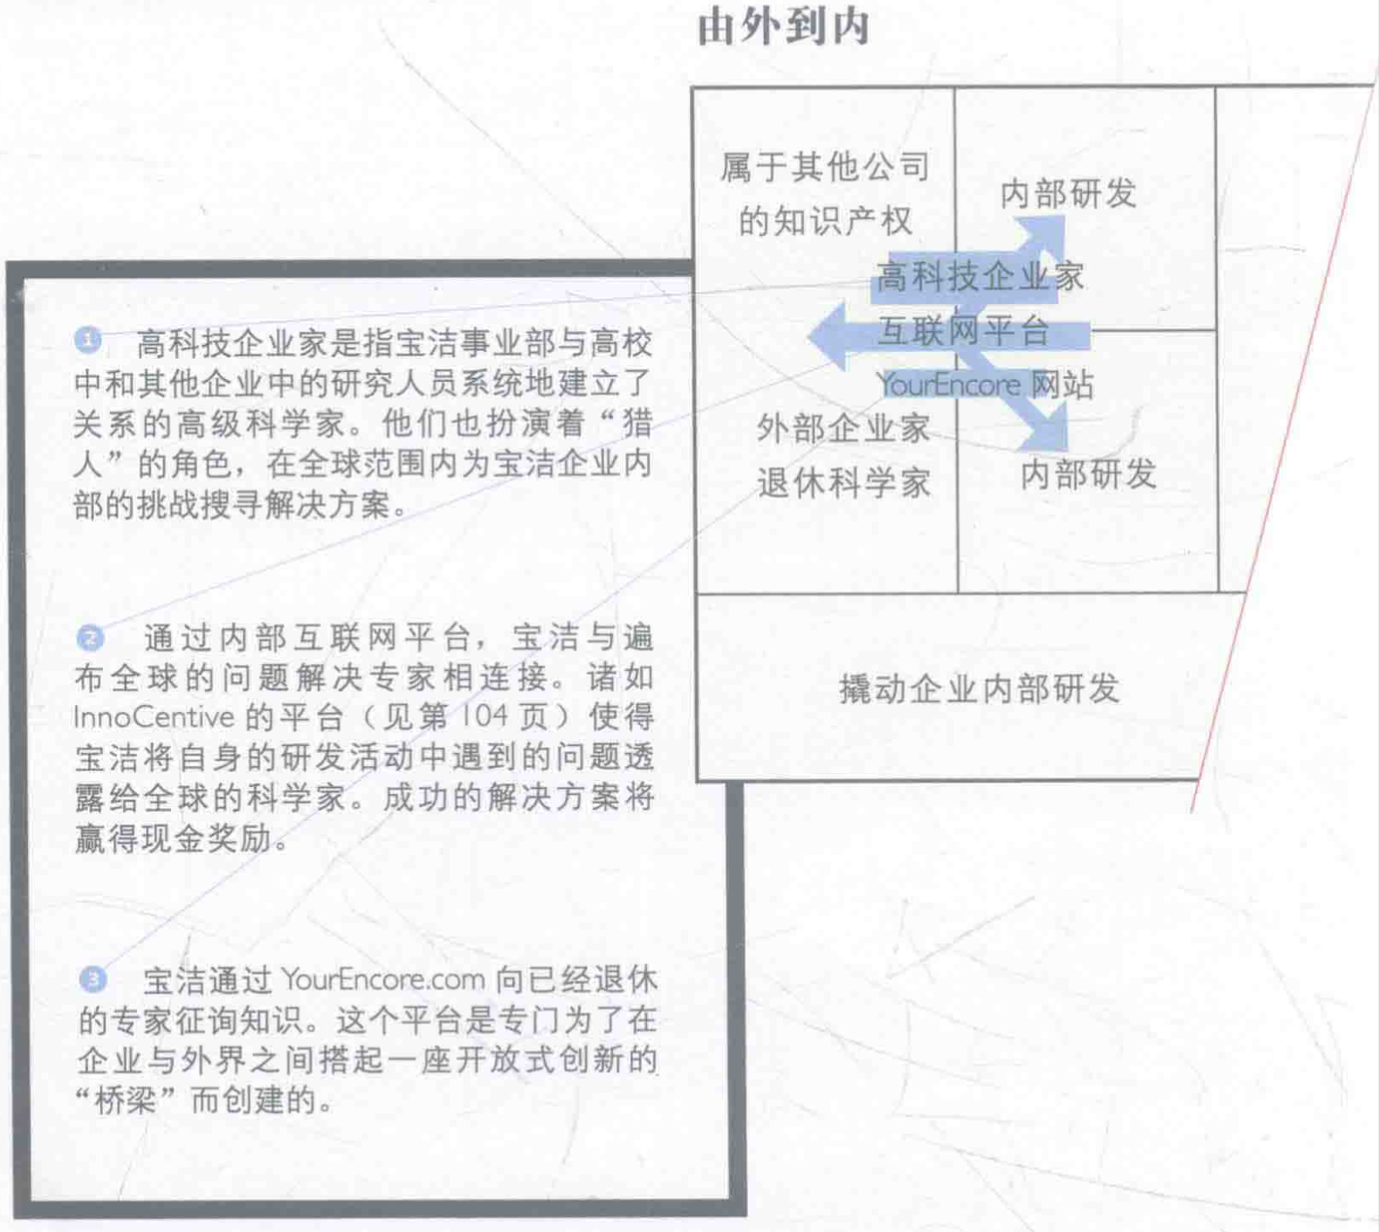
\includegraphics[width=0.6\textwidth]{img/宝洁.png}
        \vspace{-0.5em}
	\end{figure}

    \subsubsection{葛兰素史克的专利池}
    由外而内的开放式创新方法是将企业内部的闲置资产变现,主要针对专利和技术
    \begin{itemize}
        \item 葛兰素史克的目标是提高世界上最贫困国家的药物普及率,以及在研究不足的疾病领域投入更多的研发
        \item 葛兰素史克建立的专利池,主要放置和治疗疾病相关的知识产权,并对外开放,避免研发进度由个别专利人阻挠而停滞
        \begin{itemize}
            \item 停止在50个最不发达地区申请或主张专利(允许仿制)
        \end{itemize}
    \end{itemize}
    
    \begin{figure}[H]
		\centering
        \vspace{-0.5em}
		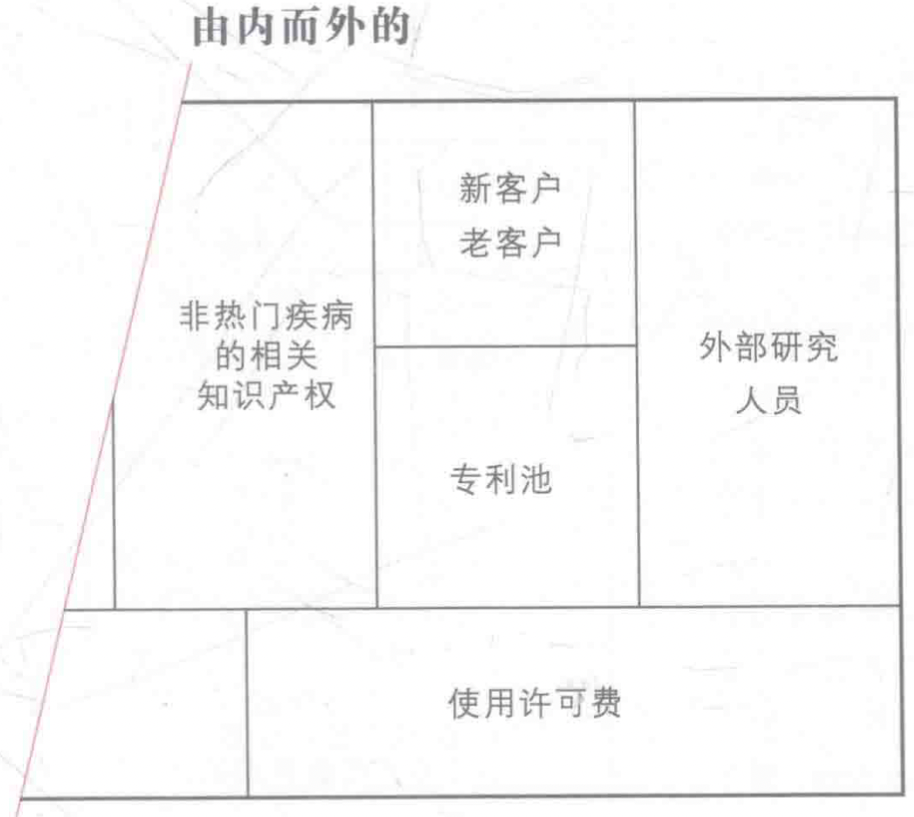
\includegraphics[width=0.4\textwidth]{img/葛兰素史克.png}
        \vspace{-0.5em}
	\end{figure}

    \subsubsection{连接器:InnoCentive}
    企业向外部的研究人员寻求灵感也有可能产生可观的成本,例如当企业有目的地吸引某些人才或企业的合作,而这些人才或企业拥有能够为其解决自身问题提供帮助的知识时。另外,当某企业的研究人员试图在该企业以外使用自己的知识时,为了找到有吸引力的机会,同样会发生搜索成本。
    \begin{itemize}
        \item InnoCentive就是为有研发问题需要解决的组织和全世界范围内有强烈意愿去解决具有挑战性的问题的研究人员提供一个连接,目前发展为一家独立的中介机构。
    \end{itemize}
    
    \begin{figure}[H]
		\centering
        \vspace{-0.5em}
		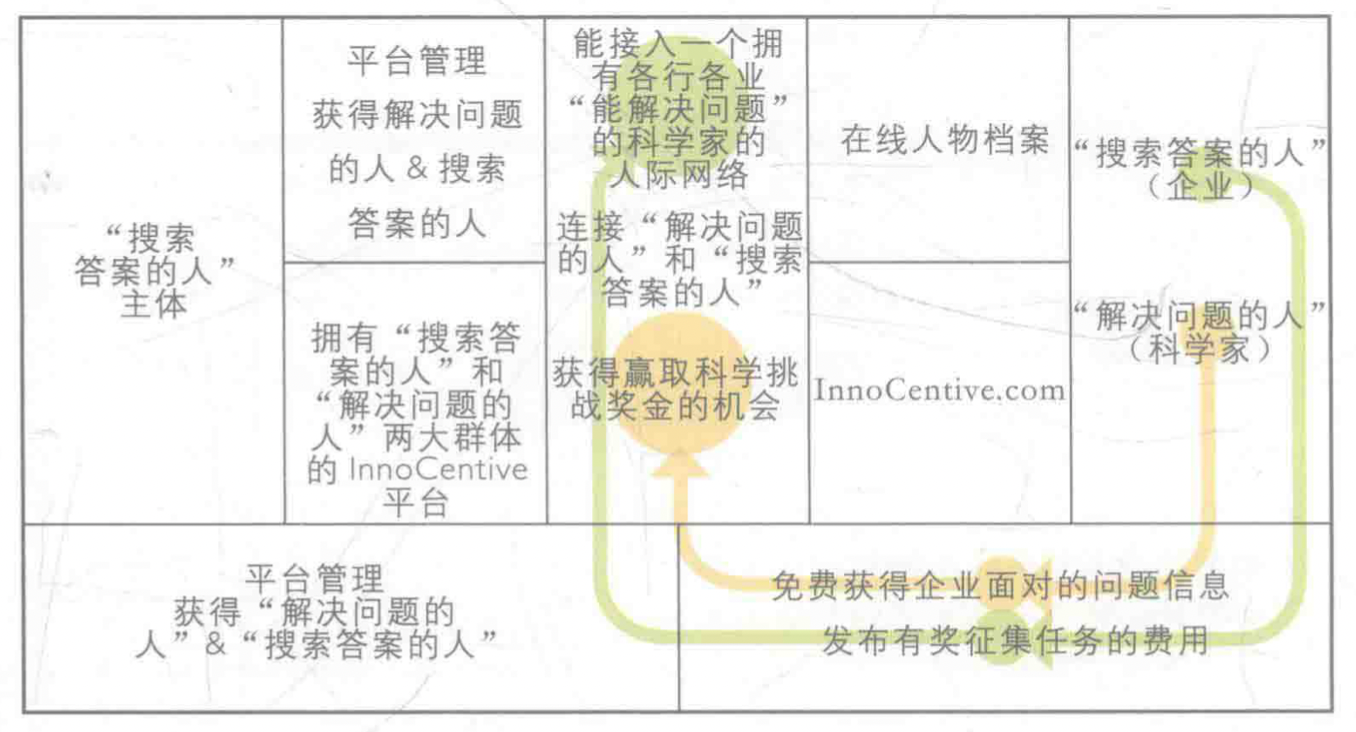
\includegraphics[width=0.6\textwidth]{img/InnoCentive.png}
        \vspace{-0.5em}
	\end{figure}

    \subsubsection{由外而内的模式总结}
    \begin{figure}[H]
		\centering
        \vspace{-0.5em}
		
\includegraphics[width=0.7\textwidth]{img/由外而内的模式.png}
        \vspace{-0.5em}
	\end{figure}
    
    \subsubsection{由内到外的模式总结}
    \begin{figure}[H]
		\centering
        \vspace{-0.5em}
		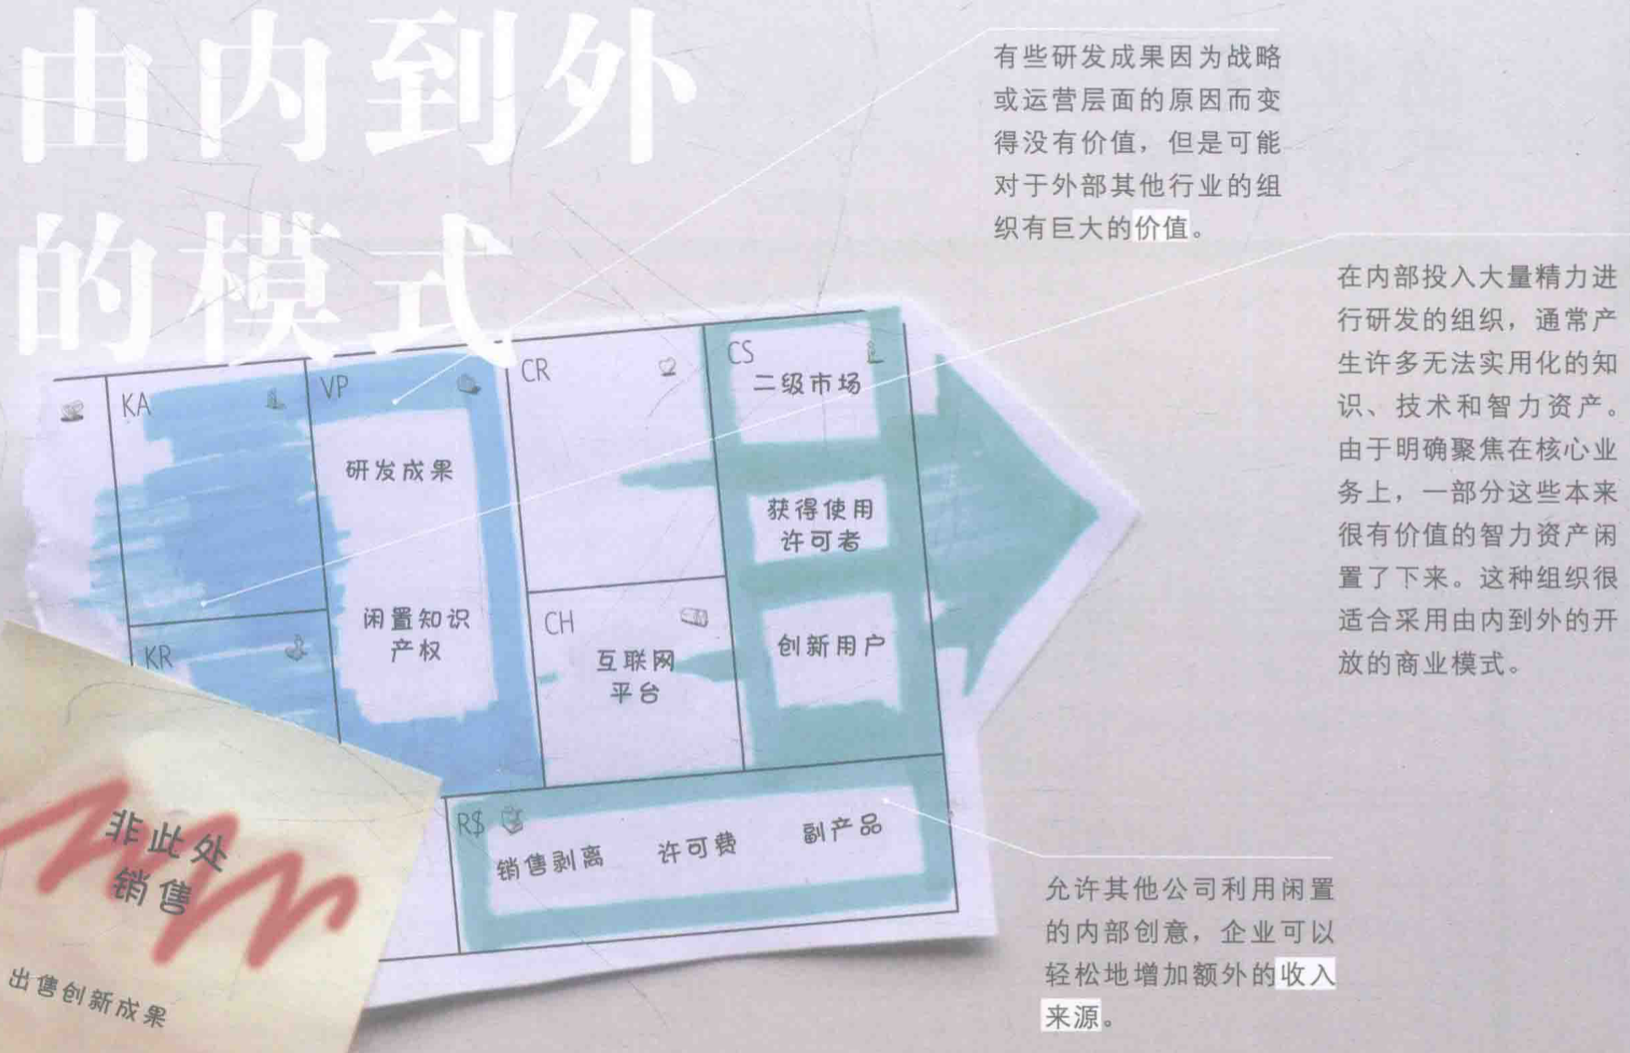
\includegraphics[width=0.7\textwidth]{img/由内到外的模式.png}
        \vspace{-0.5em}
	\end{figure}

    \subsection{商业模式类型总结}
    \begin{figure}[H]
		\centering
        \vspace{-0.5em}
		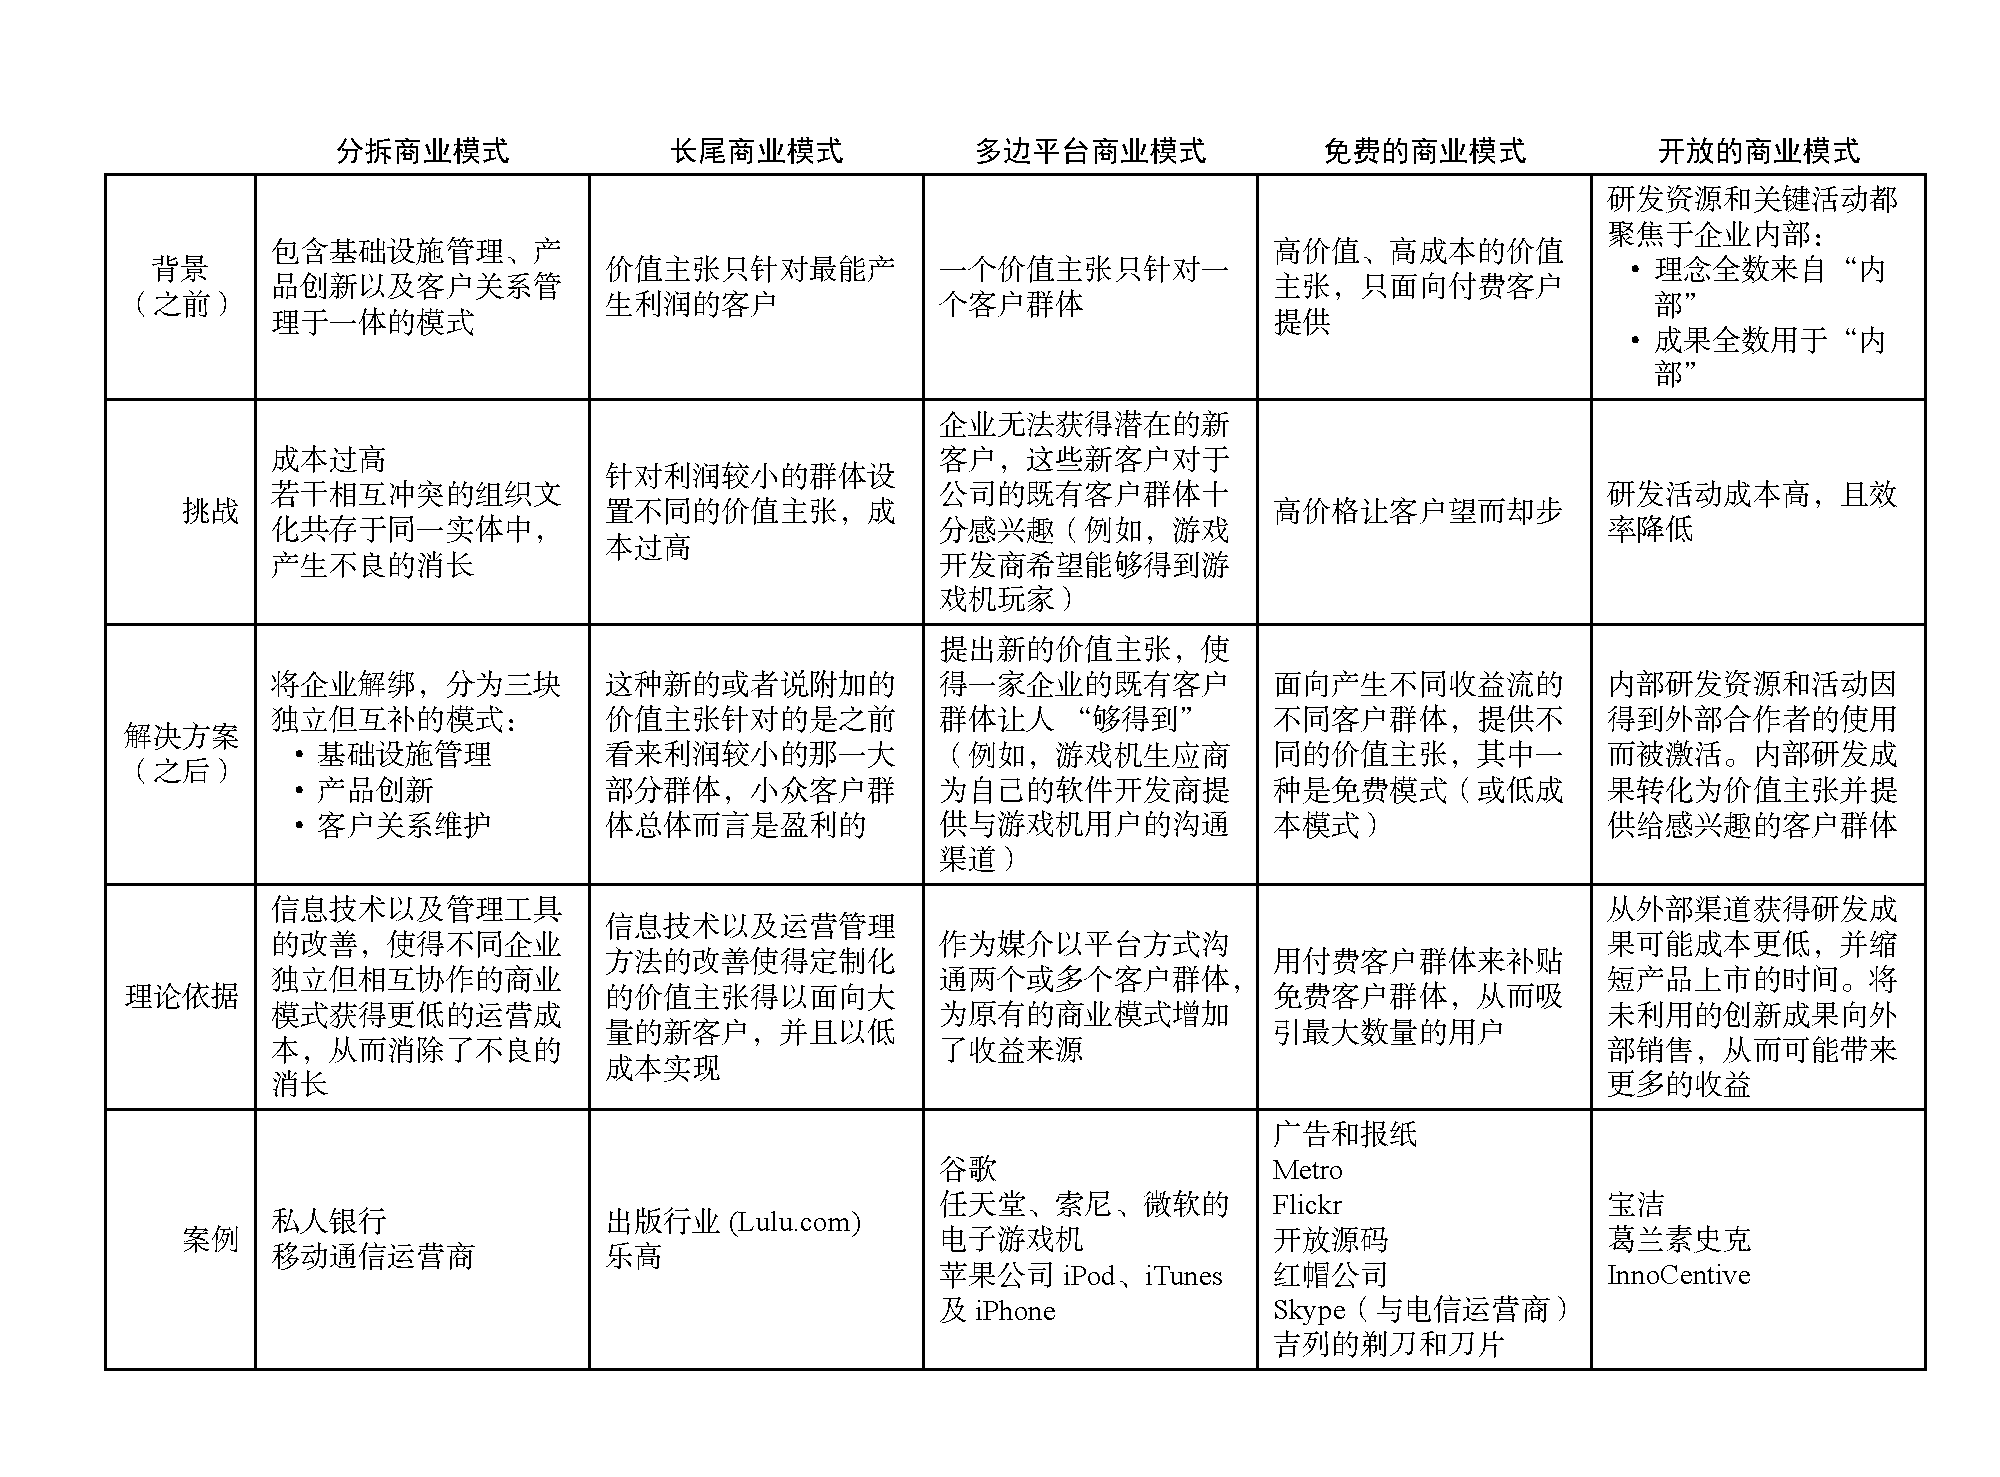
\includegraphics[width=\textwidth]{img/商业模式总结.pdf}
        \vspace{-0.5em}
	\end{figure}

















